\label{NN_proposal_chapter}
In the last chapter, some experiments were performed with the help of the implementation of Kolmogorov complexity discussed in Section \ref{Library_K_complex}. It uses the so-called Block Decomposition Method or BDM for short. This implementation showed that it can measure the complexity of sequences of bits better than any other previous method. Nonetheless, it has a high computational cost, especially for large sequences. This and the enormous amount of possible applications motivates to look for new methods to measure the K-complexity. It is desirable to have a method which can approximate algorithmic complexity for long sequences in less time.\\

In this chapter, we propose a hybrid method which uses the results obtained with the BDM for short sequences. This hybrid method is based on the combination of a method of block decomposition and non-linear regressions performed with Neural Networks. We call this method The Block Decomposition Method with Neural Networks (BDMNN). The results indicate that this method is faster than the classical BDM, though the cost is an increase in the error of the complexity computed. Therefore, for long sequences, the behavior of the BDMNN approaches to the behavior shown by the entropy method to estimate complexity. Despite this, we strongly believe that the error can be reduced with the help of more sophisticated design of the Neural Networks, the use of larger training sets, and more learning time. Thus, this first attempt of hybrid method is just the beginning in the search of a faster implementation to measure Kolmogorov complexity and its results are promissory.\\

We will begin by giving the theoretical framework behind the functioning of neural networks as functions to perform non-linear regressions. Then, the description of the methodology used to create the new method to measure complexity will be presented. Finally, some results obtained with this implementation will be discussed and compared with those obtained with the classical BDM.

\section{Theoretical Framework}
\subsection{Machine Learning}
Nowadays the use of machine learning techniques has taken increasing importance. Machine learning helps to perform all kind of tasks. It is based on the idea of teaching and learning from examples, instead of direct programming as usual. Some usual definitions are the following:

\begin{defn}
Machine Learning is the science (and art) of programming computers so they can learn from data \cite{machine_hands_on}.
\end{defn}

\begin{defn}
(Machine Learning is the) field of study that gives computers the ability to learn without being explicitly programmed \cite{machine_samuel}.
\end{defn}

When it is said that a computer learns, it means the following:
 
\begin{defn}
\label{learn_definition}
A computer program is said to learn from experience $E$ with respect to some task $T$ and some performance measure $P$, if its performance on $T$, as measured by $P$, improves with experience E \cite{machine_mitchell}.
\end{defn}

We can understand this former definition with the simplest example of a machine learning program, a spam filter. This program can determine by itself whether an email is a spam or not. To do so, it uses as examples the emails which we tag as spam. These examples constitute the so-called \textit{training set} or \textit{training data}. Thus, in this example, the task $T$ is the action of tagging the spam emails, the experience $E$ is the training data, and the performance can be, for instance, the percentage of emails correctly tagged as spam by the machine.\\

Other common examples of machine learning programs are the following: a program which uses the photo of a person to predict its age, a program which recognizes whether a Tweet is aggressive or not, a program which can classify objects in a photo, a chatbot, a voice assistant, a program which can learn to play a game, a program which finds irregular data, a program which paints works of art, etc. As can be seen, the type of data which can be managed by the machine learning techniques is immense. It can be used to work with images, time series, text, video, music, measurements, medical data, graphs, etc. Every object which can be represented as a vector, or more generally as a tensor, can be manipulated with the techniques of machine learning to perform a specific task. The task can be a classification, a prediction, a regression, a decision making, a clustering, a detection, a sorting, the estimation of a probability density, etc.\\

There are many machine learning techniques and diverse ways to classify them. The most common way to classify machine learning techniques is by the type of human supervision during the training process. In this way, we distinguish between supervised, unsupervised, semi-supervised and reinforcement learning. In supervised learning we supply the program with training data and with the desired solutions, i.e., we target the training data with the solution corresponding to each example \cite{machine_mitchell}. Conversely, in unsupervised learning, the training data does not have a labeled solution, so the program must learn without target solutions \cite{machine_mitchell}. On the other hand, semi-supervised learning combines supervised and unsupervised learning since the training data is partially labeled with the solutions \cite{machine_mitchell}. Finally,  in reinforcement learning, an agent observes the environment and creates a strategy called policy to perform an action and receive a reward in return, its objective is to maximize this reward by means of the policy chosen \cite{machine_mitchell}.\\

\begin{figure}
\centering
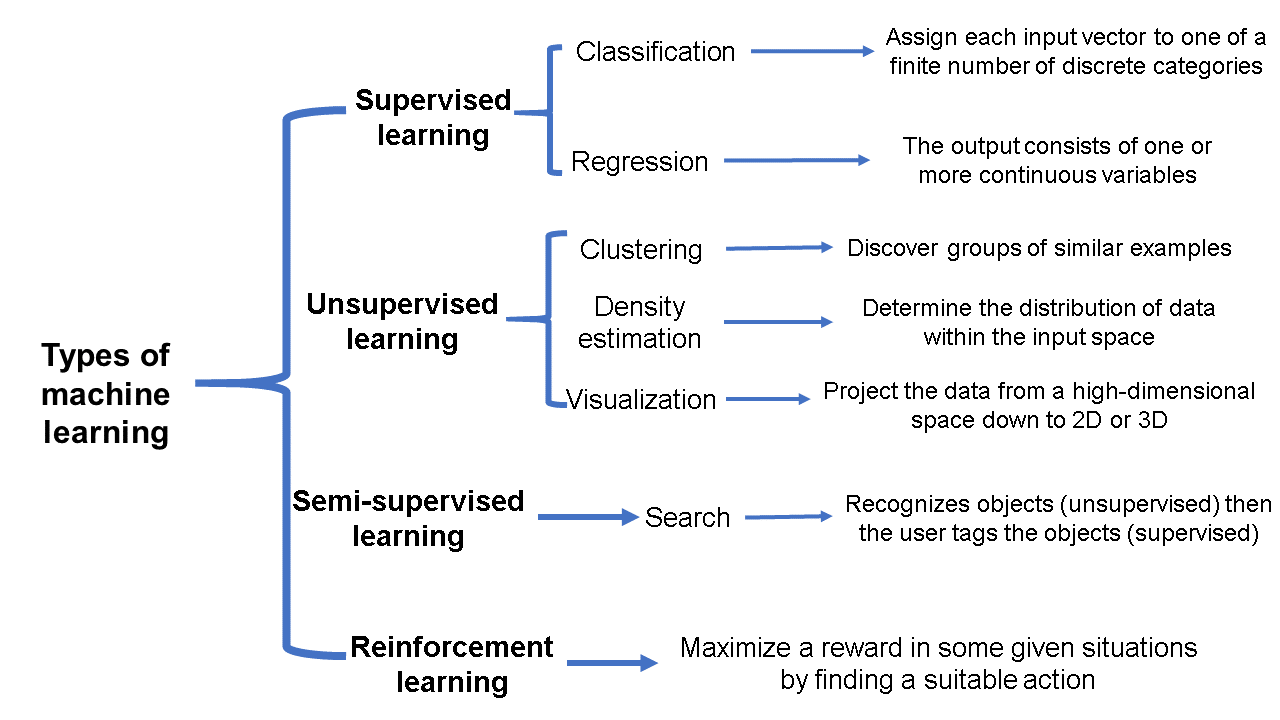
\includegraphics[width=\textwidth]{machine_types}
\caption[The types of machine learning techniques classified according to the type of human supervision during the training process and some tasks which can be performed with them.]{The types of machine learning techniques classified according to the type of human supervision during the training process and some tasks which can be performed with them \cite{machine_bishop}.}
\label{fig:machine_types}
\end{figure}

In Fig. \ref{fig:machine_types} can be seen the types of machine learning techniques and some tasks which can be performed with them. As was mentioned, every category includes distinct types of machine learning techniques which can be used for many different tasks. In this work, we are only interested in supervised learning. As was mentioned before, in supervised learning, the data we provide comprises examples with their respective labeled solutions. If the solutions (desired outputs) are a finite number of discrete categories, then the task is called classification. On the other hand, if they consist of one or more continuous variables the task is called regression \cite{machine_bishop}. This task tries to predict a target numeric value given a set of features known as predictors \cite{machine_mitchell}. For instance, we could try to predict the height of a person (the target numeric value), given its age, sex, and nationality (the predictors).\\

There many machine learning techniques to perform a regression. Among the most important techniques, we can mention k-Nearest Neighbors, Linear Regression, Logistic Regression, Support Vector Machines (SVMs), Decision Trees and Random Forests, and Neural Networks \cite{machine_mitchell}. The most appropriate technique will depend on many factors such as the type of data considered, the training speed, the accuracy desired, the memory needed to save the model, etc. Generally, the election of one model or other will depend on our experience and our knowledge and assumptions about the data. Nevertheless, the basic ideas behind all of them are the same. We provide the computer with a training set $\vec{X}= \{ \vec{x_{1}},\vec{x_{2}},...,\vec{x_{N}} \}$ and label the desired output of each example in this set with a target vector $\vec{t}= \{ t_{1},t_{2},...,t_{N} \} $. Therefore, we have a list of training examples where each element is a pair of the form $(\vec{x},t)$ which can be written for the $N$ training examples as $((\vec{x_{1}},t_{1}),(\vec{x_{2}},t_{2}),...,(\vec{x_{N}},t_{N}))=((\vec{x},t)_{1},(\vec{x},t)_{2},...,(\vec{x},t)_{N})$.\\

In the case of a regression, the output $t_{i}$ represents one or more continuous variables and the input $\vec{x_{i}}$ can be a tensor of any dimensions \footnote{Evidently, all the inputs $\vec{x_{i}}$ need to have the same dimensions, though there exist machine learning techniques were this is not necessary. On the other hand, the outputs $t_{i}$ need always to have the same dimensions to be consistent.}. Then, we perform the machine learning algorithm which returns a function $y$. This function can map new inputs $\vec{x_{new}}$ to a target value $t_{prediction}$ (the prediction), i.e., $y(\vec{x_{new}})=t_{prediction}$. Evidently, the new input and output values $\vec{x_{new}}$ and $t_{prediction}$ will have the same dimensions used during the training phase. It is common to perform a preprocessing of the input data before the training phase to make the task simpler to learn  \cite{machine_bishop}. This preprocessing is known as feature extraction, and when used before training the new data must be preprocessed as well.\\

Later in this chapter, we will choose the technique of Neural Networks to perform a regression. For this reason, in the next sections, we will briefly review this model and its training process.

\subsection{Neural Networks}
\subsubsection{The Perceptron}
\label{perceptron_section}
The artificial Neural Networks were born inspired by biological Neural Networks. These networks are made up of millions of units called neurons which are interconnected in a complex web. In artificial Neural Networks (ANNs), the precursors of the units (the neurons) used in modern multilayer networks are the \textit{perceptrons}, so we will begin the study of this unit model before considering networks with many interconnected units. Suppose we have $n$ inputs $\vec{x}= \{ x_{1},...,x_{n} \}$, then the output computed by the perceptron is the following \cite{machine_mitchell}:

\begin{equation}
\label{perceptron1}
	f(x_{1},...,x_{n})= \begin{cases}
	1 &\text{if $w_{0} +w _{1} x _{1} + w _{2} x _{2} + \cdots + w _{n} x _{n} > 0$}\\
	-1 &\text{otherwise }\\
	\end{cases}	
\end{equation}

Where each $w _{i}$ is a real-valued constant called \textit{weight} and $w _{0}$ is a bias parameter. The weight determines the contribution of each input $x _{i}$ to the output. As can be seen, the output of the perceptron depends on the linear combination $w_{0} +w _{1} x _{1} + w _{2} x _{2} + \cdots + w _{n} x _{n}$, therefore it is usual to take $w _{0}=1$ and write the linear combination as $\sum_{i=0}^{n} w _{i} x _{i} $, then in vector notation the linear combination is $\vec{w}\cdot \vec{x}$, where $\vec{w}= \{ w_{1},...,w_{n} \}$. Thus Eq. \ref{perceptron1} is rewritten as \cite{machine_mitchell}:

\begin{equation}
\label{unit_eq}
f(\vec{x})=h(\vec{w}\cdot \vec{x})
\end{equation}

This is the general equation for a unit (a neuron). The function $h$ is a nonlinear activation function, and in the case of the perceptron unit, this function is the $sign$ function which is given by:

\begin{equation}
	sgn(y)= \begin{cases}
	1 &\text{if $y>0$}\\
	-1 &\text{otherwise }\\
	\end{cases}	
\end{equation}

\begin{figure}
\centering
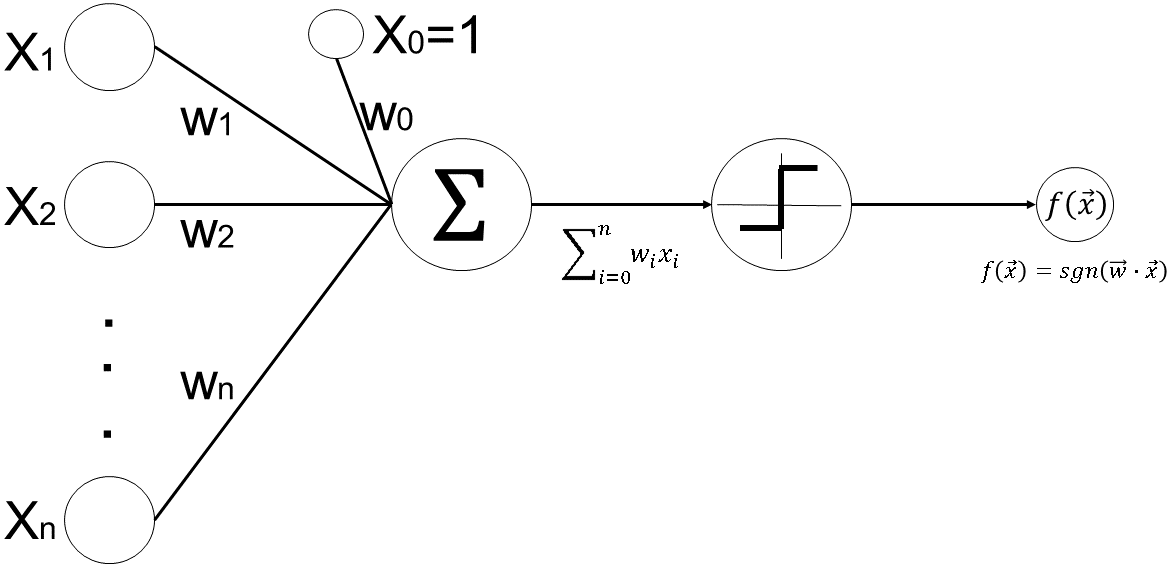
\includegraphics[width=\textwidth]{perceptron}
\caption{Graphical representation of the perceptron.}
\label{fig:perceptron}
\end{figure}

\begin{figure}
\centering
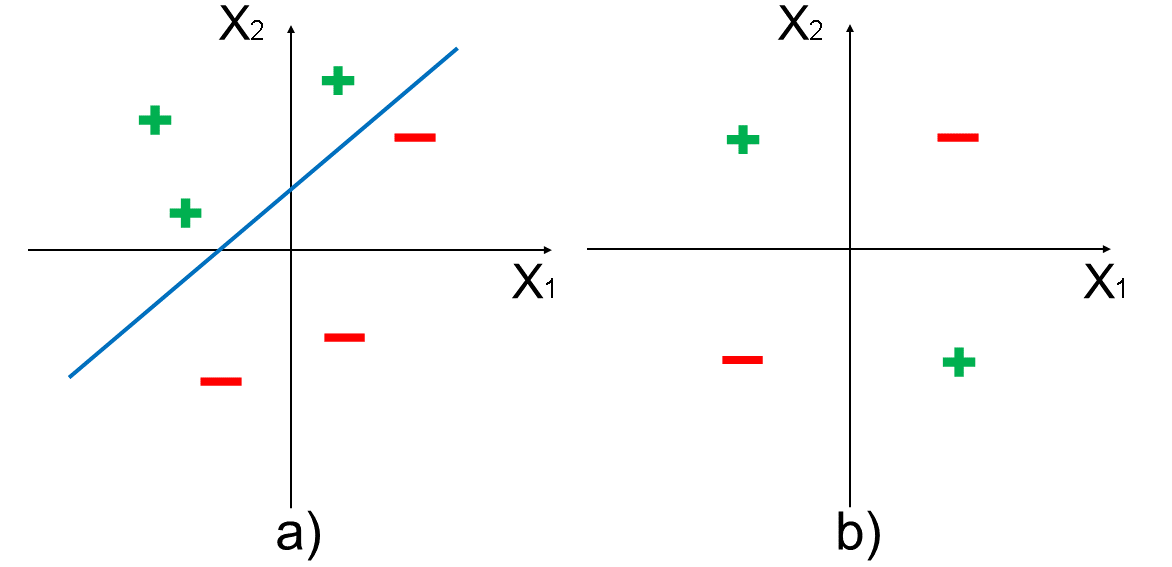
\includegraphics[width=\textwidth]{separable_perceptron}
\caption[Graphical representation of the decision surface of a perceptron with two inputs.]{Graphical representation of the decision surface of a perceptron with two inputs: $x_{1}$ and $x_{2}$.  If a set of examples is linearly separable, then it is possible to use a straight line to separate them in the decision surface. a) A set of linearly separable examples. b) The XOR function represents a set of non-linearly separable examples since its value is $1$ if and only if $x_{1} \neq x_{2}$ \cite{machine_mitchell}.}
\label{fig:separable_perceptron}
\end{figure}

In Fig. \ref{fig:perceptron} a graphical representation of the perceptron is shown. The perceptron can have two possible outputs, $1$ and $-1$. This makes the perceptron a function which can represent Boolean functions such as the basic functions AND, OR, NAND, NOR. Besides, the perceptron is said to be a linear classifier, since it can classify a set of examples into two classes, corresponding to the values $1$ and $-1$. Although, it only can classify sets of linearly separable examples, which means that it cannot represent functions like the XOR function \cite{machine_mitchell}. This is represented in Fig. \ref{fig:separable_perceptron}.\\

The behavior of the perceptron is adjusted by means of the weights $\vec{w}= \{ w_{1},...,w_{n} \}$. These parameters allow the perceptron to learn. There are different algorithms to adjust these parameters, in the following section, we will review the method of gradient descent because it is the base of other learning algorithms which even can be used to train networks with many interconnected units. Unfortunately, the gradient descent algorithm requires the nonlinear activation function $h$ in Eq. \ref{unit_eq} to be differentiable. Then, it can only be applied to a to an unthresholded perceptron where $h$ is the identity or a unit with a differentiable activation function.\\

\subsubsection{The Gradient Descent Method}
\label{Gradient_Descent_Method}
In this section, we will present the Gradient Descent algorithm to learn the weights $\vec{w}= \{ w_{1},...,w_{n} \}$ of a unit. This method can be applied to any unit of the form given in Eq. \ref{unit_eq} with the condition that the nonlinear activation function $h$ must be differentiable. In this section, for convenience, we will consider as example and unthresholded perceptron, i.e., $f(\vec{x})=\vec{w}\cdot \vec{x}$. Thus, in this section when we mention perceptron, we are referring to a perceptron whose nonlinear activation function $h$ is the identity. In this way, if the problem to solve is linearly separable, then this algorithm converges to the exact solution, however, if the problem is not linearly separable, then it converges to the best-fit for the given target set \cite{machine_mitchell}.\\

Firstly, as was mentioned in Definition \ref{learn_definition}, we need a performance measure of the learning process, i.e., we need to define an error function. There are different ways to define an error function, for a perceptron, we can define it as follows \cite{machine_mitchell}:

\begin{equation}
\label{perceptron_error}
	E(\vec{w})=\frac{1}{2} \sum_{i \in D} (t_{i}-f_{i})^{2}
\end{equation}

Where $D$ is the set of training examples, $t_{i}$ is the target output for the training example $i$, and $f_{i}$ is the output of the perceptron for the training example $i$. This error function is a function of the vector $\vec{w}$ because the output $f$ of the perceptron is a function of this vector.\\

The error function of Eq. \ref{perceptron_error} measures the discrepancy of the output produced by the perceptron while using a hypothesis weight vector $\vec{w}$, against the desired output given by the set of training examples. Therefore, if the training examples are linearly separable, we expect this function to be $0$ when a weight vector $\vec{w}$ makes the perceptron to exactly reproduce the targets of these training examples. On the other hand, in case that the training examples were not linearly separable, the best-fit approximation must occur when this function reaches its minimum value. This can be seen in Fig. \ref{fig:error_function}. Therefore, the problem of training the perceptron is the problem of finding the minimum of the error function given in Eq. \ref{perceptron_error}. In our case, this function always is parabolic with a global minimum, though in general, for networks with multiple units (and not necessarily the same kind of error function) there can exist multiple local minimums.\\

\begin{figure}
\centering
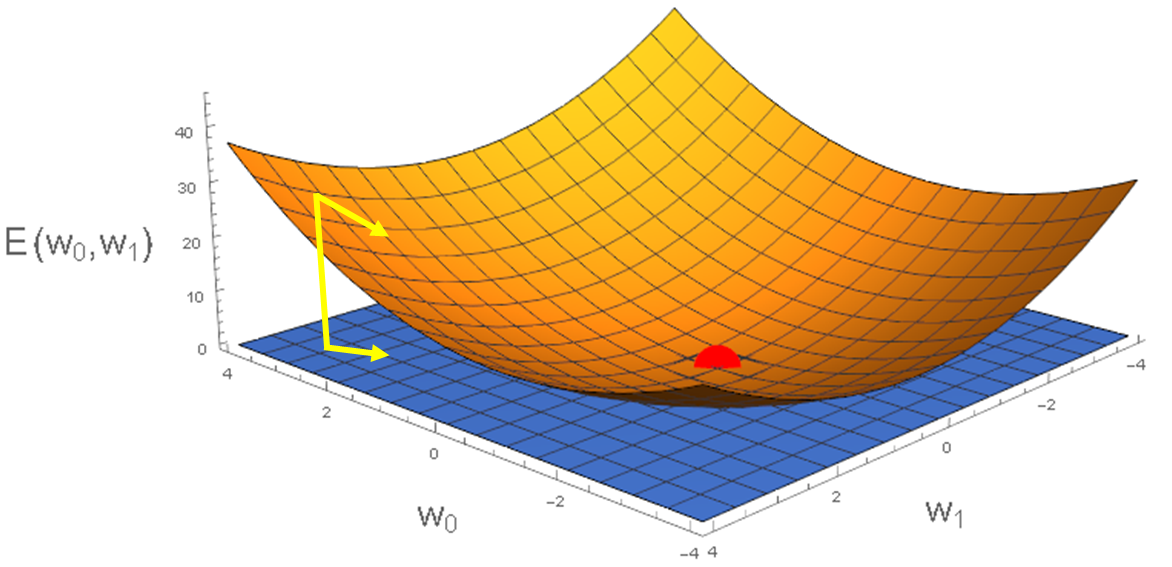
\includegraphics[width=\textwidth]{error_function}
\caption[Error surface for a perceptron with weight vector $\vec{w}= \{ w_{0},w_{1} \}$.]{Error surface for a perceptron with weight vector $\vec{w}= \{ w_{0},w_{1} \}$. The axes $w_{0}$ and $w_{1}$ create a plane which represents the possible values of the weights $w_{0}$ and $w_{1}$. The axis $E$ indicates the value of the error function. The shape of the parabola depends on the set of training examples. The arrow on the surface indicates the direction of the negative of the gradient at one particular point and its projection onto the plane $w_{0}w_{1}$ indicates the direction in this plane which produces the steepest descent along the error surface \cite{machine_mitchell}. The red point indicates the global minimum.}
\label{fig:error_function}
\end{figure}

The gradient descent algorithm searches the weight vector which minimizes the error function. The weight vector $\vec{w}$ is usually randomly initialized and at each step it is moved in the direction that produces the steepest descent along the error surface in steps of a determined size until the global minimum is reached.\\

As can be remembered, the result of the gradient is another vector which negative gives the direction of steepest decrease. Therefore, to find the direction of steepest descent along the error surface in a point, we need to compute the gradient of the error function with respect to the vector $\vec{w}$:

\begin{equation}
	\vec{\nabla} E(\vec{w})=  \Bigg \langle \frac{\partial E}{\partial w_{0}}, \frac{\partial E}{\partial w_{1}}, \ldots , \frac{\partial E}{\partial w_{n}}     \Bigg \rangle
\end{equation}

The negative of this gradient evaluated in a point $(w_{0}w_{1})$ gives the direction of steepest descent along the error surface from that point, as is shown in Fig. \ref{fig:error_function}.\\

Thereby, at each step the vector $\vec{w}$ is updated following the rule \cite{machine_mitchell}:

\begin{equation}
\label{update_rule_gradient_descent}
	\vec{w} \leftarrow \vec{w} + \triangle \vec{w}
\end{equation}

where

\begin{equation}
\label{update_rule_gradient_descent}
	 \triangle \vec{w} = -\eta \vec{\nabla} E(\vec{w})
\end{equation}

The constant $\eta$ is a positive constant called the learning rate, and it determines the step size to take in the direction of the steepest descent at each iteration. This rule can be written for each component as \cite{machine_mitchell}:

\begin{equation}
	w_{i} \leftarrow w_{i} + \triangle w_{i}
\end{equation}

where

\begin{equation}
\label{rule_component_descent}
	 \triangle w_{i} = -\eta \frac{\partial E}{\partial w_{i}} 
\end{equation}

Thus, each component $w_{i}$ is modified by an amount proportional to $\frac{\partial E}{\partial w_{i}} $. It is easy to construct an algorithm to perform the gradient descent rule by means of Eq. \ref{rule_component_descent}, we just need to compute the partial derivatives of $E$ and evaluate them at the corresponding point. From Eq. \ref{perceptron_error} it is easy to show that the partial derivative of the error function with respect to $w_{i}$ is given by:

\begin{equation}
	 \frac{\partial E}{\partial w_{i}} = \sum_{k \in D} (t_{i}-f_{i})(-x_{ik})
\end{equation}

Where $x_{ik}$ is the single input component $x_{i}$ for the training example $d$. Thus, we can rewrite Eq. \ref{rule_component_descent} as follows:

\begin{equation}
\label{rule_gradient_descent}
	 \triangle w_{i} = \eta \sum_{k \in D} (t_{i}-f_{i})x_{ik}
\end{equation}

The learning rate $\eta$ can increase the speed of the convergence, however, if its value is too large, the algorithm can get us away from the minimum instead of getting us closer. Thus, to guarantee the convergence it is necessary to use a sufficiently small value for $\eta$, especially being close to the minimum \cite{machine_mitchell}.\\

\begin{figure}
\centering
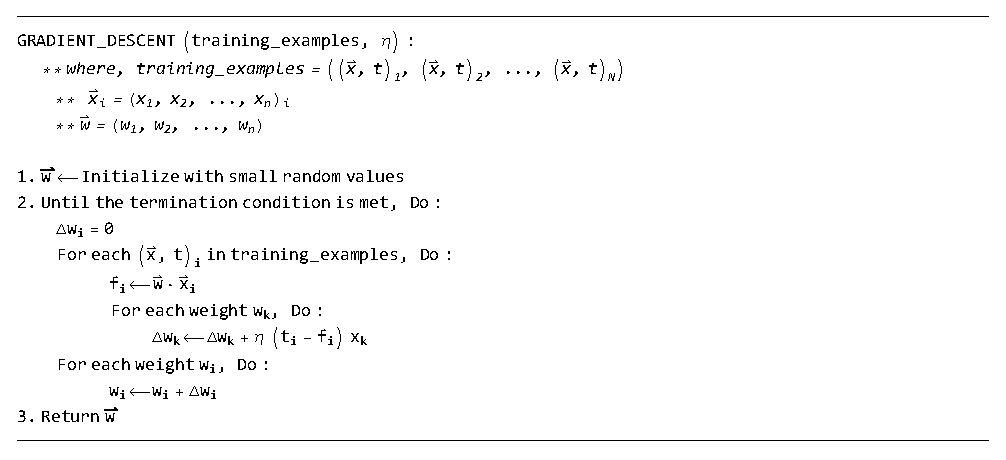
\includegraphics[width=\textwidth]{gradient_descent_algorithm}
\caption[Gradient descent algorithm for training a linear unit.]{Gradient descent algorithm for training a linear unit \cite{machine_mitchell}.}
\label{fig:gradient_descent_algorithm}
\end{figure}

The gradient descent algorithm to train a perceptron is shown in Fig. \ref{fig:gradient_descent_algorithm}. This method can be applied if the error function is differentiable with respect to the weights. Nonetheless, it may converge to the minimum quite slow, moreover, if the error surface has multiple local minima, it is not guaranteed that it will find the global minima.\\

As was mentioned before, there are many other algorithms to train a unit. These methods can overcome the difficulties encountered with the gradient descent method and fortunately, many of them are simple variations to the method presented in this section, such as the algorithm of stochastic gradient descent which will be discussed in the next section given its importance in the majority of the most important optimization methods to train Neural Networks.

\subsubsection{The Stochastic Gradient Descent Method}
The idea behind this method is to avoid the sum of Eq. \ref{rule_gradient_descent}. Instead, we consider an error function defined for each individual training example as follows \cite{machine_mitchell}:

\begin{equation}
	 E_{k}(\vec{w})=\frac{1}{2}(t_{k}-f_{k})^{2}
\end{equation}

Thus, the weights are updated using each training example $(\vec{x},t)_{k}$ following:

\begin{equation}
\label{rule_gradient_descent}
	 \triangle w_{i} = \eta (t_{k}-f_{k})x_{i}
\end{equation}

Where for the \textit{k}th training example, $t_{k}$ is the target value, $f_{k}$ is the output of the unit, and $x_{i}$ is the \textit{i}th input.\\

Therefore, in this method the search of the minimum is guided by $\nabla E_{k} (\vec{w})$ instead of $\nabla E (\vec{w})$, i.e., instead of Eq. \ref{update_rule_gradient_descent} we use $\triangle \vec{w} = -\eta \vec{\nabla} E_{k}(\vec{w})$.


\subsubsection{Feed-Forward Neural Networks}
In this section, we will see how we can combine many units (neurons) to create a multilayer network also known as Neural Network or NN for short, but first, we need to choose the kind of units which will compose the network. The former optimization methods required the activation function of the unit to be differentiable. In fact, many optimization methods demand this requirement. Hence, this is the main reason for not considering the perceptron as the basic unit for constructing a multilayer network., even though, this model played a key role in the history of machine learning \cite{machine_bishop}. Thus, it is common to build multilayer networks by considering units whose activation function is differentiable.\\

A basic Neural Network model is built with units of the form given by Eq. \ref{unit_eq}. Nonetheless, for convenience, we will establish a new nomenclature. To do so, we will describe how to build a multilayer network from the beginning. Let $\{x_{1},...,x_{D}\}$ be the input variables, then firstly, we form $M$ linear combination of these input variables as follows \cite{machine_bishop}:

\begin{equation}
\label{linear_comb_first_layer}
	 a_{j}=\sum_{i=0}^{D} w_{ji}^{(1)}x_{i}
\end{equation}

Where $j=1,...,M$. The number $M$ of linear combinations indicates that this first layer has $M$ units. The superscript $(1)$ indicates that these units are in the first layer of the network. As before, the parameters $w_{ji}^{(1)}$ are the weights (in the first layer according to the superscript). It must be remarked, that we have adopted the convention of taking the bias parameter as $w_{j0}^{(1)}=1$ with $x_{0}=1$ as we did for the perceptron. Each unit of the layer $a_{j}$ is activated through a nonlinear activation function $h^{(1)}$:
 
\begin{equation}
\label{hideen_units_first_layer}
	 f_{j}^{(1)}=h^{(1)}(a_{j})
\end{equation}

Each $f_{j}^{(1)}$ represents an activated unit which in the context of Neural Networks are known as hidden units \cite{machine_bishop}. As was said, the activation functions must be differentiable, but we will talk about the choosing process later. Equations \ref{linear_comb_first_layer} and \ref{hideen_units_first_layer} define the hidden units in the first layer, to add a new layer to the network, we follow the same procedure, i.e., we construct linear combinations of the input variables for the second layer. For the second layer these input variables are the hidden units in the first layer:

\begin{equation}
\label{linear_comb_second_layer}
	 a_{k}=\sum_{j=0}^{M} w_{kj}^{(2)}f_{j}^{(1)}
\end{equation}

Where $k=1,...,K$. The number $K$ of linear combinations indicates that this second layer has $K$ units, or in other words, the second layer has $K$ outputs. Again, we have taken the bias parameter as $w_{k0}^{(2)}=1$ with $f_{0}^{(1)}=1$. These units are also activated with a nonlinear activation function $h^{(2)}$:

\begin{equation}
\label{hideen_units_second_layer}
	 f_{k}^{(2)}=h^{(2)}(a_{k})
\end{equation}

Thus, up to now, we have constructed a Neural Network with two layers (we will not consider the input variables of the first layer as units). The function of this Neural Network is:

\begin{equation}
\label{NN_feed_forward}
	 f_{k}^{(2)}(\vec{x},\vec{w})=h^{(2)} \bigg( \sum_{j=0}^{M} w_{kj}^{(2)} h^{(1)} \bigg( \sum_{i=0}^{D} w_{ji}^{(1)}x_{i} \bigg) \bigg)
\end{equation}

\begin{figure}
\centering
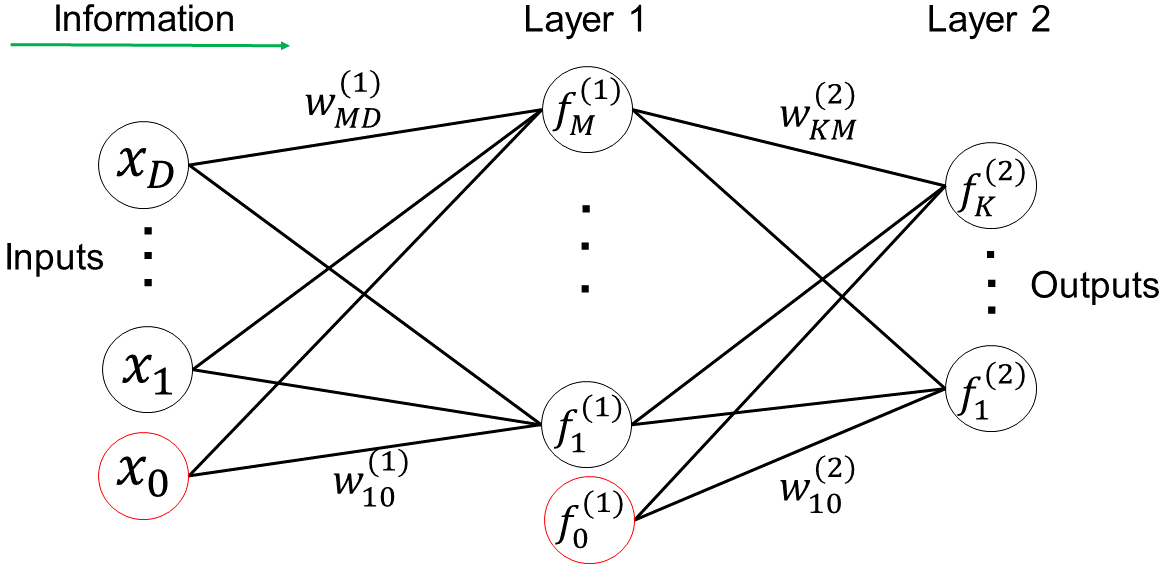
\includegraphics[width=\textwidth]{multilayer_network}
\caption[The topology of a feed-forward Neural Network with two layers.]{The topology of a feed-forward Neural Network with two layers. The information flows through the network in the direction indicated by the green arrow. The nodes of the graph indicate the input variables, the hidden units (first layer) and the output units (second layer). The edges of the graph indicate the weight parameters. The red nodes indicate the hidden variables whose edges are the bias parameters. The layers which are not input or output layers are known as hidden layers. In this case, we have a single hidden layer, the first layer.}
\label{fig:multilayer_network}
\end{figure}

Thereby, a Neural Network model is simply a nonlinear function of the input variables $\vec{x}$ and the weights $\vec{w}$ with the set of outputs $\{ f_{k}^{(2)} \}$. The topology of the Neural Network defined by Eq. \ref{NN_feed_forward} can be represented by the graph shown in Fig. \ref{fig:multilayer_network}. This type of topology is said to be fully connected since every node transfers information to every node in the next adjacent layer \cite{deep_learning}. Evidently, this is not the only kind of possible topology, but it is one of the most common and is easily generalized, besides it is the topology we will use later in this chapter. This type of topology for a Neural Network is known as feed-forward Neural Network since the process of evaluating is a forward propagation of information through the network \cite{machine_bishop}. This model is also known as multilayer perceptron because it resembles the perceptron model discussed in Section \ref{perceptron_section}, nevertheless, the perceptron uses an activation function which is not differentiable, whereas the Neural Network uses differentiable activation functions. Thus, the function of a Neural Network is differentiable with respect to the network parameters which is important for network training.\\

The Neural Network defined by Eq. \ref{NN_feed_forward} has two layers, however, the process described in this section can be repeated to add as many layers as we wish. The $k$th output of a Neural Network with $m$ layers can be represented by the following equation:

\begin{equation}
\label{NN_feed_forward_full}
	 f_{k}^{(m)}(\vec{x},\vec{w})=h^{(m)} \bigg( \sum_{j=0}^{M} w_{kj}^{(m)} h^{(m-1)} \bigg( \sum_{i=0}^{Q} w_{ji}^{(m-1)} h^{(m-2)} \bigg( \cdots \bigg( \cdots h^{(1)} \bigg( \sum_{q=0}^{D} w_{qp}^{(1)}x_{p} \bigg) \bigg)  \bigg) \bigg) \bigg)
\end{equation}

Hence, it is possible to imagine a Neural Network with $m$ layers simply as a composition of functions:

\begin{equation}
	f_{k}^{(m)}(\vec{x},\vec{w})= h^{(m)}(f_{k}^{(m-2)}(f_{k}^{(m-1)}( \cdots ( f_{k}^{(1)}(\vec{x},\vec{w})))))
\end{equation}

Where $f_{i}(\vec{x},\vec{w})= h^{(i)} (\sum_{j} w_{ij}^{(i-1)} x_{j}) $, and the sum runs over all units which send information to unit $i$, including the bias parameter. This way to see the system is important since it means we can compute the derivatives of the Neural Network by means of the chain rule.\\

\subsubsection{Feed-forward Neural Networks as Approximators}
\label{nn_power}
The model described by Eq. \ref{NN_feed_forward_full} seems to be quite complex, so it is expected it will be a great model to perform approximations. In fact, Neural Networks are said to be universal approximators \cite{machine_bishop}. We have some theorems regarding several types of functions:

%\begin{quote}
%A two-layer network with linear outputs can uniformly approximate any continuous function on a compact input domain to arbitrary accuracy provided the network has a sufficiently large number of hidden units (\cite{machine_bishop}, page 230).
%\end{quote}

\begin{theorem}[Boolean Functions]
Every Boolean function can be represented exactly by some network with two layers of units, although the number of hidden units required grows exponentially in the worst case with the number of network inputs (\cite{machine_mitchell}, page 105).
\end{theorem}

\begin{theorem}[Continuous Functions]
Every bounded continuous function can be uniformly approximated on a compact input domain with arbitrarily small error (under a finite norm) by a network with two layers of units provided the network has a sufficiently large number of hidden units. The units must have a sigmoid activation function at the hidden layer and (unthresholded) linear units at the output layer (\cite{machine_mitchell}, page 105; and \cite{machine_bishop} page 230).
\end{theorem}

\begin{theorem}[Arbitrary Functions]
Any function can be approximated to arbitrary accuracy by a network with three layers of units. The output layer must have linear units, and the two hidden units must have units with a sigmoid activation function. The number of units required at each layer is not known in general (\cite{machine_mitchell}, page 105).
\end{theorem}

\subsubsection{Network Training}
\label{backpropagation}
In this section, we will present the Backpropagation algorithm to train the weight parameters of a multilayer network with a fixed set of units and interconnections. This algorithm is based on the Gradient Descent Method studied in Section \ref{Gradient_Descent_Method}. Therefore first, we need to define an appropriate error function. To do so, we will generalize the error function presented in Eq. \ref{perceptron_error} to consider the error over all the network output units \cite{machine_mitchell}: 

\begin{equation}
\label{multilayer_error}
	E(\vec{w})=\frac{1}{2} \sum_{i \in D} \sum_{k \in outputs} (t_{ki}-f_{ki})^{2}
\end{equation}

Here, $outputs$ is the set of output units of the network, $t_{ki}$ is the target output for the training example $i$ in the $k$th output unit, and  $f_{ki}$ is the output of the network in the $k$th output unit for the training example $i$.\\

Thus, as was argued in Section \ref{Gradient_Descent_Method}, the problem of learning the weight parameters is the problem of minimizing the error function of Eq. \ref{multilayer_error}. This error function can be visualized by an error surface like the one shown in Fig. \ref{fig:error_function}. Nonetheless, now this space is defined by the error function defined in Eq. \ref{multilayer_error} and the weight parameters of all the units in the multilayer network. The idea is the same, we need to find the values of the weight parameters which minimize the error function, i.e., we need to find the minimum of the error surface. Therefore, we can use the gradient descent method to find the minimum. However, this time the error surface can have multiple local minima, so the convergence towards the global minimum is not guaranteed.\\

The idea is the same, we randomly initialize the weight parameters and compute the gradient of the error function. The negative of the vector given by the gradient will indicate the direction of steepest descent along the error surface in that given point. Then, we update the weight parameters according to $w_{ji} \leftarrow w_{ji} + \triangle w_{ji}$. Following the same procedure of Section \ref{Gradient_Descent_Method}, we can compute the gradient of the error function and obtain the rule to update the value of the weights. We will not show it here, but the gradient descent weight-rule is given by \cite{machine_mitchell}:

\begin{equation}
\label{backpropagation}
	 \triangle w_{ji} =-\eta \nabla E(\vec{w}) = \eta \delta_{j} x_{ji}
\end{equation}

Where $\eta$ is the learning rate, $ x_{ji}$ is the input value to which the weight is applied, and $\delta_{j}$ is given by:

\begin{equation}
\label{rule_gradient_descent}
	 \delta_{j} =  \eta f_{j} (1-f_{j})  \sum_{k \in Downstream(j)} \delta_{k} w_{kj}
\end{equation}

Here, $Downstream$ denotes the set of units whose direct inputs include the output of unit $j$. This last equation shows that the value of $\delta$ for a hidden unit is obtained by propagating backward the $\delta$ values from units higher up in the network. This is the reason for the name backpropagation.\\

There are other algorithms to train the parameters of a multilayer network which follow immediately as variations of the rule given in Eq. \ref{backpropagation}, nevertheless, we will not consider its details since it lies out of our reach. In practice, we only need to know the convergence properties of each method to choose one to solve a specific task.

\subsubsection{Designing the Network}
The design of a Neural Network to solve a specific task is an art which only can be learned with the experience. However, there are certain rules which can be used as a starting point.\\

The number of input units will be given by the dimensionality of the network, e.g., if our input data are 1-D vectors whose length is $8$, then the number of input units will be $8$ plus a unit for the bias parameter. In the same way, the number of output units will be given by the expected output of our model. For instance, if we perform a regression, then the output of the network will be a scalar which means the number of output units will be $1$. On the other hand, if for example, our model gives as output the presence or the absence of a cat and/or a dog in an image, then it would be adequate to use two output units. An output unit which gives the presence or absence of the cat and another which gives the presence or absence of the dog.\\

The number of hidden units must be adjusted to give the best predictive performance; however, we need to have in mind that more layers mean more units which also means more parameters to be trained. Therefore, it is necessary to get a balance between a good predictive performance and the training time needed to reach it. If we need to perform a regression, we can see from the theorems presented in Section \ref{nn_power} that usually two hidden layers will suffice for most of the problems. The number of units in these hidden units also must be adjusted to give the best balance between performance and training time. Even though it is possible to use the number of inputs units as the number of units in the hidden layers, this is not recommended \cite{fudamentals_deep_learning}. It is a better practice to have fewer units in the hidden layers than in the input layer to force the network to learn compressed representations of the original input. This does not mean that using the same number of units in the input layer and in the hidden layers will give bad results, however, it is possible that in this way we are introducing redundancy in our model which do not contribute to enhancing its performance and just makes larger the computational time needed to train the network.\\

Moreover, it is not required to connect every unit (neuron) with all the units in the next layer, i.e., the fully connected topology shown in Fig. \ref{fig:multilayer_network} is not a demand when designing the network. However, again it is an art the election of which neurons will be connected to another neuron \cite{fudamentals_deep_learning}.\\

\begin{figure}
\centering
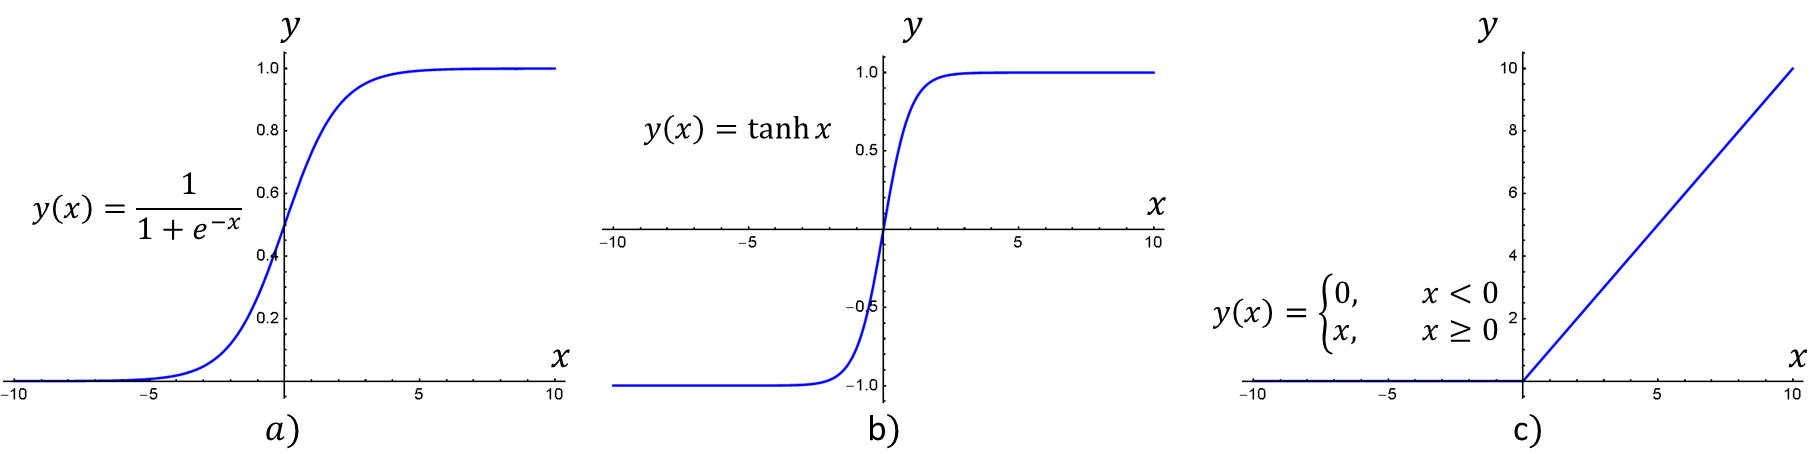
\includegraphics[width=\textwidth]{activation_functions}
\caption[The most commonly used activation functions for the units of multilayer networks.]{The most commonly used activation functions for the units of multilayer networks. a) The Logistic Sigmoid function, b) The Hyperbolic Tangent function, and c) The Rectified Linear Unit function (ReLU).}
\label{fig:activation_functions}
\end{figure}

\begin{figure}
\centering
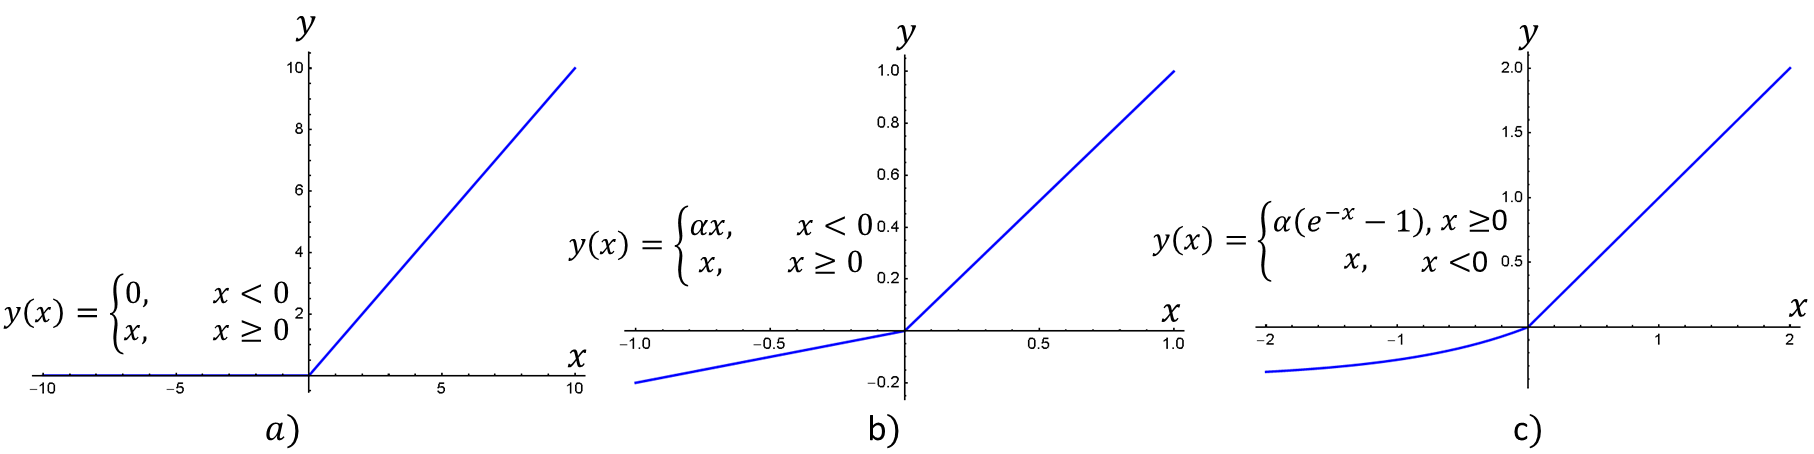
\includegraphics[width=\textwidth]{relu_variants}
\caption[Some of the most common variations for the Rectified Linear Unit function (ReLU).]{Some of the most common variations for the Rectified Linear Unit function (ReLU) \cite{relu_online} \cite{act_fun_online}. a) The ReLU function. b) The Parametric ReLU function (PReLU) (in this function the slope $\alpha$ is given to the network as a parameter to be learned. When this parameter is fixed with the value $\alpha=0.01$, this function is known as Leaky ReLU). c) The Exponential Linear Unit.}
\label{fig:relu_variants}
\end{figure}


As can be remembered, the activation functions introduce non-linearities to the multilayer networks which allow them to represent almost any arbitrary function. The election of the activation function for the units depends on whether the unit belongs to a hidden layer or an output layer, in the specific task of the model, and in the expected performance. In the hidden layers, the most commonly used activation functions are: Sigmoid (or Logistic), Tanh (Hyperbolic Tangent), and Rectified Linear Unit (ReLU) (and its variants) \cite{deep_learning}. These activation functions can be seen in Fig \ref{fig:activation_functions}. Every activation function has its advantages and disadvantages, nevertheless, the ReLU activation function or its variants are usually chosen for most of the tasks \cite{fudamentals_deep_learning}, some variants of this function have been created to solve some drawbacks in the training process (see Fig. \ref{fig:relu_variants}).\\

In the case of the output layers, the election of the activation functions is driven by the type of output expected. For regression problems, we use a linear activation function, i.e., $y(x)=x$. For binary classification, we use a single neuron with a sigmoid function which delivers a probability distribution for a single class (the probability of the other class is $(1-p)$). For multiclass classification we use the so-called \textit{SoftMax output layer} (also known as SoftMax layer) which uses the outputs of all the units in the output layer to compute a probability distribution for each output unit as follows \cite{fudamentals_deep_learning}:

\begin{equation}
y_{i}=\frac{e^{x_{i}}}{\sum_{j} e^{x_{j}}}
\end{equation}

Where the sum of all the outputs fulfils $\sum_{j} e^{x_{j}}=1$. A perfect prediction will give an output from the SoftMax layer with the probability value of $1$ while the other outputs will have a probability value of $0$, indicating that this output is the class predicted by the model. An imperfect prediction will give several values for each output. The class will be indicated by the output with the highest probability value.\\

We finish this section by commenting that there are other types of Neural Networks which can be used to solve determined types of tasks more efficiently, like the Convolutional Neural Networks or the Recurrent Neural Networks, though we will not consider them here.

\subsubsection{Choosing the Error Function}
As we saw before, the error function measures the performance of the Neural Network while using some set of weight parameters with respect to a given a set of training examples, i.e., it measures the misfit between the output of the network and the corresponding target in the training data set. This function, which is minimized by the optimizer to get the best performance, is also known as the loss function. We will use the terms error function and loss function as synonyms.\\

In Eq. \ref{multilayer_error} we defined an error function, nevertheless, there are many other possible error functions which may be more appropriate to use depending on the type of task to solve and the nature of the data. Here we will review some of the most frequently used error functions. In our notation, we will use $f$ to indicate the output of the network, $t_{i}$ to indicate the target of the $i$th sample in the training set, and $N$ to indicate the number of samples in the training set. Finally, $t_{ij}$ will indicate the output of the $j$th output unit obtained with the $i$th sample of the training set.

\subsubsection*{Loss Functions for Regression}
These loss functions can be used when the task to solve is a regression problem. The most popular is the \textit{Mean Squared Error Loss (MSE)} function, which is given by \cite{deep_learning}:

\begin{equation}
\label{MSE}
	E(\vec{w})=\frac{1}{N} \sum_{i =1}^{N} (f_{i}-t_{i})^{2}
\end{equation}

This function resembles the error function used to perform the ordinary least squares in linear regression, but here we divide the sum by the number of training samples. This function is mainly used to perform regression when the output is a real value, i.e., a scalar. If the output is a vector of size $M$, or in other words, if the outputs are $M$ continuous variables, then the former loss function is generalized as \cite{deep_learning}:

\begin{equation}
	E(\vec{w})=\frac{1}{N} \sum_{i =1}^{N} \frac{1}{M}  \sum_{j =1}^{M} (f_{ij}-t_{ij})^{2}
\end{equation}

Note that Eq. \ref{MSE} is the especial case where $M=1$. For convenience this function is sometimes modified as \cite{deep_learning}:

\begin{equation}
	E(\vec{w})=\frac{1}{2N} \sum_{i =1}^{N} \sum_{j =1}^{M} (f_{ij}-t_{ij})^{2}
\end{equation}

An alternative to the MSE function is the \textit{Mean Absolute Error (MAE) Loss} function \cite{deep_learning}:

\begin{equation}
	E(\vec{w})=\frac{1}{2N} \sum_{i =1}^{N} \sum_{j =1}^{M} |f_{ij}-t_{ij}|
\end{equation}

When the target value has a spread of values the model can be rudely affected by the outliers. To avoid so, we use the \textit{Mean Squared Logarithmic Error (MSLE) Loss} function \cite{deep_learning} \cite{choose_fun_online}:

\begin{equation}
	E(\vec{w})=\frac{1}{N} \sum_{i =1}^{N} \sum_{j =1}^{M} (log(f_{ij})-log(t_{ij}))^{2}
\end{equation}

Finally, another possible error function is the \textit{Mean Absolute Percentage Error (MAPE) Loss} function \cite{deep_learning}:

\begin{equation}
	E(\vec{w})=\frac{1}{N} \sum_{i =1}^{N} \sum_{j =1}^{M} \frac{100 \times |f_{ij}-t_{ij}| }{t_{ij}}
\end{equation}

The choice of the loss function for regression problems will depend mainly on the type of data. For most of the cases, the MSE and MAE functions will suffice. However, when the data vary largely in range, the MSLE and MAPE functions should be considered.

\subsubsection*{Loss Functions for Classification}
These functions are used when we need to classify data into categories. For binary classification, the most commonly used loss function is the \textit{Hinge Loss} function which is given by \cite{deep_learning}:

\begin{equation}
	E(\vec{w})=\frac{1}{N} \sum_{i =1}^{N} max(0,1-t_{ij} \times f_{ij} )
\end{equation}

This function categorizes the data as $-1$ or $1$. If we are interested in the probability of belonging to a given class, more than a raw classification,  then we are interested in logistic regression. The most common function for such cases is the \textit{Cross-Entropy} function, also known as \textit{Logarithmic loss} function \cite{machine_bishop} \cite{choose_fun_online2}:

\begin{equation}
	E(\vec{w})=-\sum_{i =1}^{N} [t_{i} log (f_{i}) + (1-t_{i}) log(1-f_{i}) ]
\end{equation}

This function can be extended to consider the classification of $M$ classes (multiclass classification) \cite{machine_bishop}:

\begin{equation}
	E(\vec{w})=-\sum_{i =1}^{N} \sum_{j =1}^{M}  [t_{ij}  log (f_{ij})]
\end{equation}

\subsubsection{Choosing the Optimization Method}
In Section \ref{Gradient_Descent_Method}, we had the first contact with the Gradient Descent Method, and in Section \ref{backpropagation}, we saw how to apply it to multilayer networks. Nevertheless, this method has the disadvantage of being quite slow. The training process could take less time if we choose to use a faster optimization method. The most common and faster optimizers are the following: Momentum optimization, Nesterov Accelerated Gradient, AdaGrad, RMSProp, Adam optimization, and Nadam optimization. As was mentioned in Section \ref{backpropagation}, we cannot describe its details here since it lies out of our reach. Nevertheless, we can always safely choose to use Adam and Nadam methods. These methods are more powerful and usually converge faster than any other method since they combine ideas from other optimization algorithms (\cite{machine_hands_on}, page 293). The Nadam optimization method is an improvement to Adam optimization method, so if possible, we must give preference to Nadam over the Adam method \cite{nadam}.

\subsubsection{Regularization Techniques}
When training a Neural Network, we minimize the loss function by evaluating the given training set. We could think that the closer the value of the loss function to $0$, the better the model we get. However, we need to have in mind, that the purpose of our model is not to exactly reproduce the training data but to generalize its behavior to brand new data. We already know the behavior of the training data, so it is not interesting to build a model which exactly reproduces it. Instead, we would like to have a model which can generalize the behavior of the training data to unknown data. Therefore, it is not a clever idea to let the network learn to reproduce exactly the training data. This problem of producing a model that performs well on the training data but generalizes poorly to new data is known as overfitting (\cite{data_sience}, page 142).\\

The problem of overfitting is shown in Fig. \ref{fig:overfitting}. Suppose that we generate random data from the function $Sin(x)$ by introducing some random noise as shown in Fig. \ref{fig:original_data}. Then, we use this random data as training data for a Neural Network. If we let the Neural Network overfit the training set, then we will get a model like the one shown in Fig. \ref{fig:overfitted_data}. This model reproduces almost exactly the training data; however, it is far from the original model from which the data was generated. Thus, we can say that the overfitted model has learned the random noise in the training data, so this model is not capable of generalizing new data to the original model $Sin(x)$. Nevertheless, if we use a technique to avoid the overfitting, we can get a model which is more similar to the original model, even though, the training set is not perfectly adjusted as shown in Fig. \ref{fig:non_overfitted_data}.\\

\begin{figure}
	\centering
	\begin{subfigure}[b]{0.6\textwidth}
		\centering
		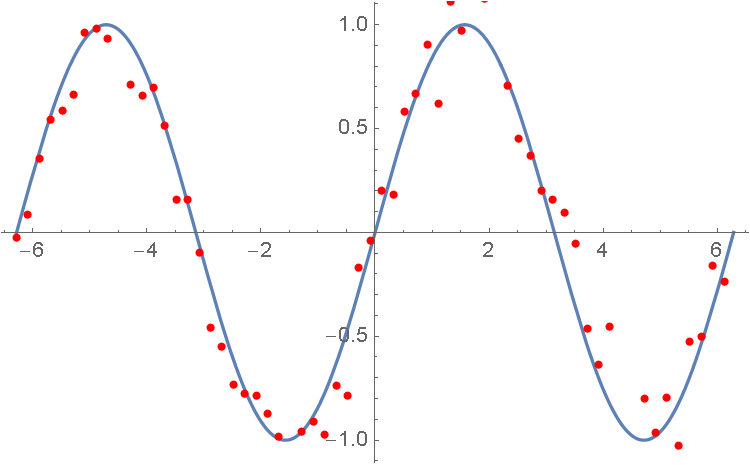
\includegraphics[width=\textwidth]{original_data}
		\caption{}
		\label{fig:original_data}
	\end{subfigure}
	%\hfill
	\hspace{0.001mm}
	\begin{subfigure}[b]{0.6\textwidth}
		\centering
		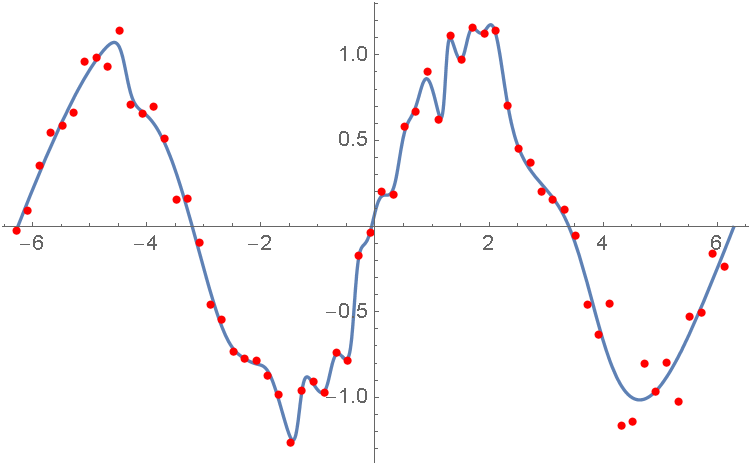
\includegraphics[width=\textwidth]{overfitted_data}
		\caption{}
		\label{fig:overfitted_data}
	\end{subfigure}
	\hspace{0.001mm}
	\begin{subfigure}[b]{0.6\textwidth}
		\centering
		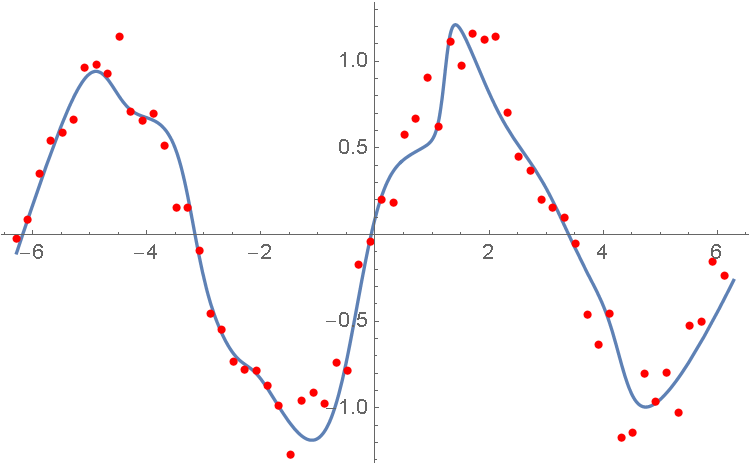
\includegraphics[width=\textwidth]{non_overfitted_data}
		\caption{}
		\label{fig:non_overfitted_data}
	\end{subfigure}
	\caption[Overfitting of a Neural Network.]{(a) Random data (red dots) obtained from introducing random noise to the function $Sin(x)$ (blue curve). (b) A Neural Network was trained by using the previous random data as training data. No method was used to avoid overfitting, so the model obtained has learned the noise of the training data and shows overfitting. (c) The same previous Neural Network was trained by using the same previous random data as a training set, but this time a validation set was used as a method to avoid overfitting. The model obtained does not show overfitting to the training data and reproduces better the original function $Sin(x)$ from which the data was obtained.}
	\label{fig:overfitting}
\end{figure}

Fortunately, there exist some techniques to avoid the overfitting of the training data. The most common technique is to reserve a portion of the training data as test data while using the rest to train the network. This test data will be used to evaluate the model in an independent way to the optimization process which is driven by the training data. In this way, we can stop the training process when the error in the test data stops decreasing and starts to increase which means the model is beginning to overfit to the training set. The test data allow us to see how well the model generalizes on new unknown data (\cite{fudamentals_deep_learning}, page 29).\\

Additionally, it is usual to divide the training process into epochs. An epoch is a single iteration over the entire training set. Moreover, the optimization process is not performed with all the training data at the same time. Instead, we perform the optimization process by using batches with a determined size obtained from the training data \cite{epoch_online}. The reason behind this can be better understood through an example: suppose we have a training set with a million of images as training samples, then the time needed to optimize the model by evaluating the error obtained with each one of these images would be immeasurable. Thus, it is better to perform the optimization process by using mini-batches (subsets) of the training data at each iteration of the optimization process. This approach allows to use the hardware resources more efficiently (\cite{deep_learning}, page 201). The performance of the model is measured at the end of each one of these mini optimization processes using the test data. However, we would also like to measure the performance of the model at the end of each epoch. Therefore, it is also usual to reserve another portion of the original training data as validation data. This validation set is used to measure how well the model is generalizing to new data at the end of each epoch (\cite{fudamentals_deep_learning}, page 29). If the error in the training data continues decreasing but the error in the validation data stays the same or starts to increase, then it means we should stop the training process because the model has begun to overfit the training data.\\

In summary, we split up the original data set into three sets:  the training data,  the test data, and the validation data.  The training data is supplied to the optimizer in batches. The validation data is used to measure the performance of the model on new data at the end of each mini-optimization process. Finally, the validation data is used to measure the performance of the model at the end of each epoch. This method is quite successful, so it is widely used (\cite{machine_mitchell}, page 111).\\

Another common technique to avoid overfitting is \textit{Dropout}. The idea is simple, at every training step, every neuron in the network (excluding the output neurons) has a probability $p$ of being temporarily turned off (\cite{machine_hands_on}, page 304). This means that at that training step, the neuron is not used in the process of optimization, but it may be turned on during the next step. The parameter $p$ which controls the activation of the neurons is called the dropout rate. This kind of parameters which control the distribution of the model parameters, and thus, the optimization and model selection during the training process are known as hyperparameters (\cite{machine_bishop} page 30, and \cite{deep_learning} page 150). This algorithm is quite successful in increasing the training speed and boosting the accuracy of the resulting model (\cite{deep_learning}, page 200). This method prevents the neuron to adapt to its neighbors by obligating it to rely less on them and by making it independent and useful by its own. What is really happening here, is that by ignoring some neurons at each training step, we are evaluating different topologies. These architectures share some neurons with their respective weights. Therefore, the resulting model is an average of the behavior of these topologies (\cite{fudamentals_deep_learning} page 34, and \cite{machine_hands_on} page 305).\\

The last technique which will be considered here is the \textit{early stopping}. This technique consists in stopping the training process when the error with respect to the validation data set stops decreasing (\cite{machine_hands_on}, page 303). This allows obtaining a model which has a good generalization performance (\cite{machine_hands_on}, page 259).\\

There exist more regularization techniques to avoid overfitting, however, we will not consider them here. Better performance can be obtained by combining the use of different regularization methods at the same time (\cite{machine_hands_on}, page 303).

\subsection{Machine Learning Frameworks}
The techniques and methods we have reviewed in this section are already implemented in many machine learning frameworks. Thus, we do not have to spend time programming the algorithms and we can simply focus on the design and deployment of our models. Among the best and most common libraries to implement machine learning methods we can name: \textit{Scikit-learn}, \textit{TensorFlow}, and \textit{Keras}. These libraries can be easily installed and used in any Python distribution and altogether with other famous packages for scientific computing in Python like \textit{NumPy}, \textit{SciPy}, \textit{matplotlib}, \textit{pandas}, etc., they make very easy and intuitive the programming and training of models like multilayer Neural Networks (see \cite{data_sience} chapter 25, \cite{machine_hands_on} chapter 9, \cite{machine_python} chapter 1, \cite{Python_datsci_Handbook} page 343, and \cite{fudamentals_deep_learning} chapter 3).

\section{Methodology}
The hypothesis behind our implementation is that the computational time needed to compute the approximation of the K-complexity with the Block Decomposition method can be significantly reduced by creating a function which imitates the behavior of the results delivered by the BDM. In other words, if we could build a function to perform a regression from some examples computed with the BDM. Therefore, once we have built this function, its evaluation could be immediate, so we could predict the complexity of new data just by performing simple arithmetic operations without the needed of performing an intricate algorithm every time we need to evaluate the complexity of a new sequence. The computational time would be absorbed in the process of creation of this function. Fortunately, this process only would need to be performed one time. Thereby, we could save a lot of time by recycling this computation. Nonetheless, the function to perform a regression of the K-complexity must be a very complicated non-linear function. Hence, it should be impossible to build it with simple regression techniques such as linear regression. Nevertheless, machine learning provides powerful techniques to perform non-linear regressions which could be used instead.  For instance, a Neural Network can be used as a powerful non-linear regression model. Therefore, given the complexity of the problem, it was decided to use this model to perform the regression.\\

Therefore, our implementation to measure the K-complexity was built in two stages. First, three Neural Networks are individually trained with examples of complexities computed with the Block Decomposition Method. Each Neural Network is specialized in predicting the complexity of sequences of bits over a given range of lengths. The second stage consists in the creation of a function which accepts sequences of any length  (sequences which length can be even larger than the initial sequences used to train the Neural Networks) and returns an approximation of Kolmogorov complexity. The previous is achieved by means of a method similar to the original Block Decomposition Method. Once we have this function, we will only have to evaluate it every time we wish to compute the complexity of a sequence, which makes it faster than the original BDM. The stages of the methodology proposed are shown in Fig. \ref{fig:methodology}. In the following sections, the details of these stages will be presented.

\begin{figure}[h]
	\centering
		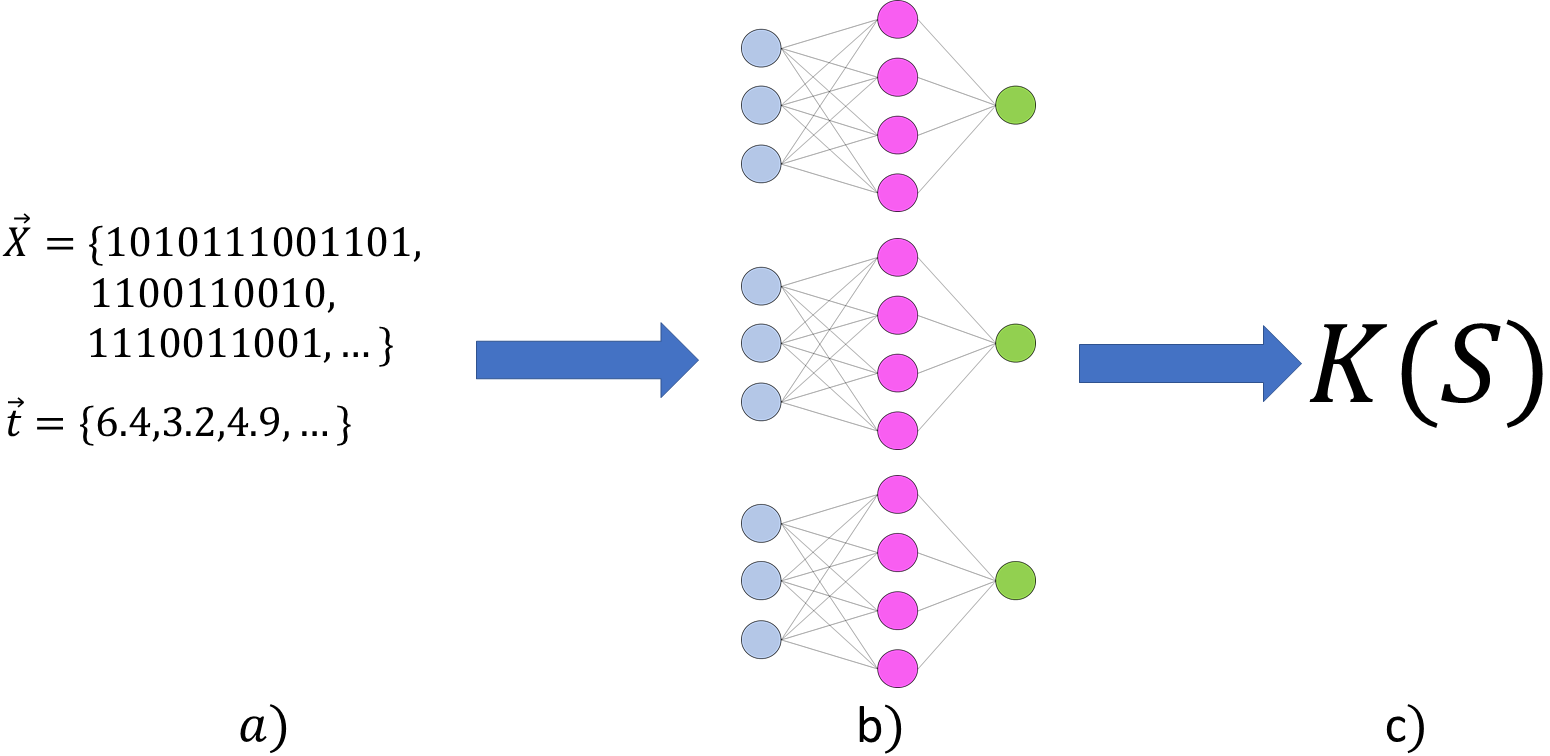
\includegraphics[width=\linewidth]{methodology}
	\caption[Stages of the methodology used to create a faster implementation to approximate K-complexity.]{Stages of the methodology used to create a faster implementation to approximate K-complexity. a) Some random sequences of bits are randomly generated, and its complexity is measured by means of the BDM. The random sequences form the training set $\vec{X}$ and its complexities the target vector $\vec{t}$. b) The training data is used to train three Neural Networks which perform a regression to approximate the algorithmic complexity of sequences of bits. Each Neural Network is specialized in approximate the K-complexity of sequences of bits between a given range of lengths. c) The three Neural Network models can be used to predict the complexity of new sequences of bits. If the new sequence has a length which lies out of the range used to train any of the three Neural Networks, the sequence is decomposed into blocks to approximate its complexity. Thus, this method resembles the original Block Decomposition Method, so we have decided to name it the Block Decomposition Method with Neural Networks (BDMNN). The details of these stages are presented in the text.}
	\label{fig:methodology}
\end{figure}

\subsection{Software and Hardware Features}
The most widely used language to program machine learning techniques, especially Neural Networks, is Python. In this language, we can find many frameworks which make fast and easily the task of implementing Neural Networks in just a few lines of code, so we only have to worry about the design and training of the models. For this reason, all the codes of this section will be written in Python Language, specifically in Python 3. The framework chosen to build and train the Neural Networks was the library \textit{Keras}. This library is user-friendly and allows to rapidly build and train Neural Network models in an intuitive way.\\

To train the Neural Networks, we needed sequences of bits whose complexity was known a priori (as will be described in the next section). Therefore, we had to rely again on the implementation of Kolmogorov complexity discussed in Section \ref{Library_K_complex}. Nevertheless, this time we are interested in the Python version of this implementation which can be downloaded from the same page\footnote{\textit{www.algorithmicdynamics.net/software.html}}. This library contains the function \textit{BDM} which can compute the 1-D and the 2-D versions of the Block Decomposition method, though we only will use the 1-dimensional version in this chapter. It accepts as argument an array (specifically a NumPy array) of $0's$ and $1's$ of length greater or equal to $12$ and returns an approximation to the algorithmic complexity of the sequence.\\

All the algorithms were implemented on the Platform \textit{Colaboratory}\footnote{https://colab.research.google.com} of Google (Google Colab) since it provides immediate access to most of the frameworks for machine learning and executes Python code in the cloud by using virtual machines. The virtual machines can be executed using GPUs instead of CPUs which makes possible to train Neural Networks faster than with a common local machine, even though they are recycled every certain amount of time so the Neural Networks can be trained in a continuous way only for a few hours.\\

\subsection{The Training and Target Sets}
One of the main complications when training Neural Networks is the amount and quality of the data used as training examples. Fortunately, in our case, we can generate and provide as many examples as we wish.\\

The procedure is very similar to the one used in Section \ref{complex_seqs_section} to generate random sequences of bits. First, we establish the maximum and minimum lengths that can have the sequences to generate. Then, we randomly (with a uniform probability) choose a length $L$ in this closed interval $[L_{min},L_{max}]$ of maximum and minimum lengths. This will be the length of the sequence to generate. Moreover, we randomly (with a uniform probability) choose a number between the interval $[0,1]$. This former number will be the probability parameter $p$ to control the complexity of the sequence generated. Afterward, we generate a sequence of length $L$, where each element has a probability $p$ of being $1$ and a probability $(1-p)$ of being $0$. Finally, the complexity of this sequence is computed by means of the BDM implementation. This algorithm is repeated a given number of times and the data generated is saved in two vectors (implemented as lists in Python). The sequences generated are stored in a vector $\vec{x}$ and its complexities in a vector $\vec{t}$. The vector $\vec{x}$ is the training vector and the vector $\vec{t}$ is the target vector.\\

The training data must be a representative sample of the possible input sequences; thus, it is important to provide as many examples as possible, but also is important ensure a uniform election of these examples among all the possible input sequences. Nevertheless, in our procedure to generate the random sequences, the cases where the sequences are only composed of $1's$ seldom occur since they appear almost only when the parameter $p$ equals $1$. To overcome this problem, we increase the frequency of apparition of these rare cases simply by rounding of the parameter $p$ to $1$ when it is greater than $0.95$.\\

Finally, once we have all the sequences and its complexities, we perform a padding procedure to fill the sequences which length was less than the maximum length. We append the value $-1$ at the beginning of each sequence until the sequence a length equal to the maximum length. In this way, for instance, if we have the sequence $\{0,1,1,0,1\}$ and the maximum length is $8$, then the padding procedure would produce the sequence $\{-1,-1,-1,0,1,1,0,1\}$. Therefore, if the complexity of the original sequence before the padding was $K(S)$, we assign to the padded sequence this same complexity $K(S)$. The final vector $\vec{x}$ with the padded sequences and the vector $\vec{t}$ with the complexities assigned to the padded sequences are the vectors which will be used to train the Neural Network.\\

The code to generate the training and target sets as described above can be found in the Appendix Section \ref{codes_python} (Fig. \ref{fig:training_data}). We generated the data to train three Neural Networks. The intervals for the length of the initial sequences (before the padding) were $[L_{min},L_{max}]=[12,20]$,$[21,100]$ and $[101,1001]$. In the three cases, the number of training examples generated was $30,000$.

\subsection{Design of The Neural Networks}
Neural Networks are widely used to solve classification problems, however, with the correct design, they also can be used to solve regression problems. They are not the only machine learning technique which can be used to perform a regression task, nevertheless, it is expected that the function which estimates Kolmogorov complexity will be highly complicated to approximate, thus, we believe that a Neural Network with the appropriate design should be able to give good results. The previous follows from the theorems presented in Section \ref{nn_power}. Nonetheless, the question of whether this is the best approach still open, though we will no try to answer this question here. Finally, the design of a Neural Network is an art since there is no standard procedure to build its topology. Our design was based on common practices.\\

The design of the three Neural Networks used in this work was the same. The only difference was the number of neurons present in each layer. The number of sequential dense layers used was $3$. The first layer had a number of neurons equal to the length of the final sequences (the maximum length) and the activation function used was the Exponential Linear activation function (ELU). This activation function has the form $f(x)=x$ for $x \geq 0$ and $f(x)=\alpha (e^{x}-1)$ for $x <0$ (the value of the parameter $\alpha$ was chosen to be $1$). The second layer had a number of neurons equal to $\dfrac{2}{3}$ times the length of the final sequences (the maximum length) and its activation function also was the ELU function. The parameter $\alpha$ also was chosen to be $1$ for this layer. The final layer only had one neuron and a linear activation function, i.e., $f(x)=x$.\\

\begin{figure}[h]
	\centering
		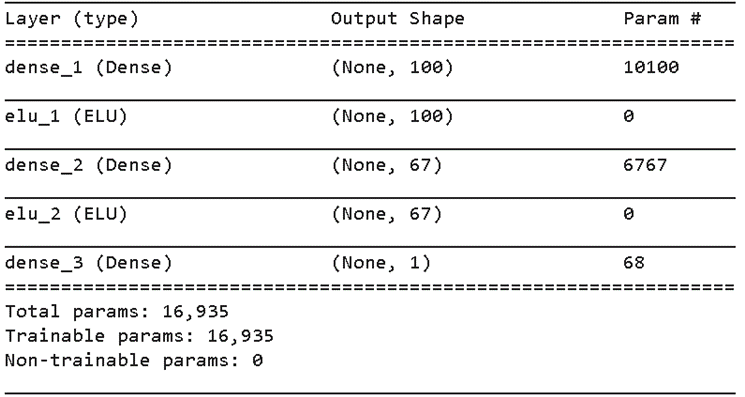
\includegraphics[width=\linewidth]{nn_design_summary}
	\caption[Summary of the design of the Neural Network which predicts the K-complexity of binary sequences.]{Summary of the design for the Neural Network which predicts the K-complexity for sequences of length between $21$ and $100$. The number of parameters to train increases with the number of layers and units, i.e., with the number of neurons.}
	\label{fig:nn_design_summary}
\end{figure}

In Fig. \ref{fig:nn_design_summary}, the summary of the design of one of the three Neural Networks built is shown. The code to build the Neural Network using the library  Keras is shown in the Appendix Section \ref{codes_python} (Fig. \ref{fig:nn_design_code}).

\subsection{The Learning Settings}
The method used to perform the optimization of the parameters of the Neural Networks was the Nesterov adaptive moment estimation optimizer (Nadam). This method usually converges to the optimal solution faster than other methods like the stochastic gradient descent method. The loss function chosen was the Mean Squared Error Loss function. The batch size used was $20$, and the entire data set was shuffled before making the batches with this size. We used a validation set to check at each epoch the accuracy of the model to data it has not seen. This validation set was randomly chosen among the training data and its size was $20 \%$ the size of the original training set. As shown in Fig. \ref{fig:nn_design_summary}, the number of trainable parameters increases with the number of units (neurons), so the time of training on each epoch also increases, besides, the number of epochs to reduce the validation error also increases. Thus, the number of epochs used to train each Neural Network was different. For the Neural Network which predicts the K-complexity of sequences which length is in between $12$ and $20$ the number of epochs was $2500$, for the Neural Network which predicts the K-complexity of sequences which length is in between $21$ and $100$ the number of epochs was $3000$ and finally, for the Neural Network which predicts the K-complexity of sequences which length is in between $100$ and $1001$ the number of epochs was $2500$. To avoid overfitting of the model to the training data, it is usual to establish a dropout parameter, which says the percentage of neurons to be off on each epoch. Nonetheless, in this case, it was not necessary to perform the dropout procedure.


\subsection{The Block Decomposition Method with Neural Networks}
Once we have performed the training of the Neural Network models, they can be used to predict the complexity of new sequences. Nevertheless, each Neural Network was trained to predict the complexity of sequences whose size is in between a given range of maximum and minimum lengths. In order to get the prediction of a new sequence which length is in between this interval, it is necessary to perform the same padding procedure used before in the generation of the training examples, i.e., we append the value $-1$ at the beginning of the sequence until it has a length equal to the maximum length. It is not possible to provide the Neural Network with sequences whose size is different since it is built and trained to only accept sequences with this feature.\\

Therefore, by using the three Neural Networks which we trained, it is possible to predict the K-complexity of sequences whose length lies in between the range $12$ and $1001$. Nonetheless, we would like to have a unique function which can predict the Kolmogorov complexity of any sequence, no matter its size. For this reason, we implemented a modified version of the Block Decomposition Method by using the three Neural Network models trained.\\

The idea is to take advantage of the three Neural Networks trained with sequences of specific lengths to predict the complexity of sequences of any size. The algorithm is the following. If the sequence we need to measure its complexity has a size which lies in between the range of sizes accepted for one of the three Neural Network models, then we simply use this Neural Network to predict the complexity of the sequence. However, if the sequence we need to approximate its complexity has a size which lies out of the range of sizes accepted for the three Neural Network models, then we perform a Block Decomposition Method, similar to the one described in Section \ref{BDM_section}. For example, if the sequence has a size longer than the maximum length of $1001$, then we split this sequence into block sequences of length equal or less than $700$. Finally, the complexity of these block sequences is measured with the corresponding Neural Network model and the complexity of the initial sequence is obtained by summing the individual complexities of these block sequences following the Eq. \ref{bdm_eq}. In our case, we have chosen to always split the original sequence into non-overlapping sequences of length equal or less than $700$. If the sequence is not a multiple of $700$, then there will be a remainder. This remainder was chosen to be ignored if its length is less than $12$ and we just simply assign to it a complexity value of $2.285794$ which is the minimum complexity which can have any sequence (see \cite{faibles_complexites}), otherwise we measure its complexity using the corresponding Neural Network. We call this method the Block Decomposition Method with Neural Networks (BDMNN) in analogy with the original BDM.\\

The code use to define the function described above is presented in the Appendix Section \ref{codes_python} (Fig. \ref{fig:def_fun_kolmo_code}). In the following section, the results of some experiments implementing this function will be shown.

\section{Results}
The implementation described above was tested by performing some experiments concerning the complexity of random sequences of bits. These experiments and its results will be shown up next. 

\subsection{The Complexity of Random Sequences of Bits}
This experiment is based on the experiment performed in Section \ref{complex_seqs_section}, but obviously, this version is implemented in Python instead of Mathematica, so there are some slight changes. First, we select the length of the sequences of bits to be generated. After, we set the probability parameter $p=0$ and begin a loop. At each iteration of the loop, we generate a sequence of bits of the length chosen initially\footnote{This time we will not generate several sequences with the same $p$ value to compute its complexity and obtain a mean value as was did in Section \ref{complex_seqs_section}. We only generate a sequence for each $p$ value.}. As can be remembered, the parameter $p$ controls the complexity of the sequence generated, since each element in the generated sequence has a probability $p$ of being $1$, and a probability $(1-p)$ of being $0$. This parameter is increased in an amount $dp$ at the end of each iteration until it reaches the value of $1$. The complexity of the generated sequence is measured by means of the original BDM implementation and our BDMNN implementation.\\

As was mentioned, this is the same experiment is basically the same that the experiment performed in Section \ref{complex_seqs_section}. Therefore, BDM implementation must show the same behavior shown in Fig. \ref{fig:random_seqs}. On the other hand, we expect BDMNN to show similar behavior to BDM, which would mean that our method is also a good approximation to Kolmogorov complexity. \\

\begin{figure}[h]
	\centering
		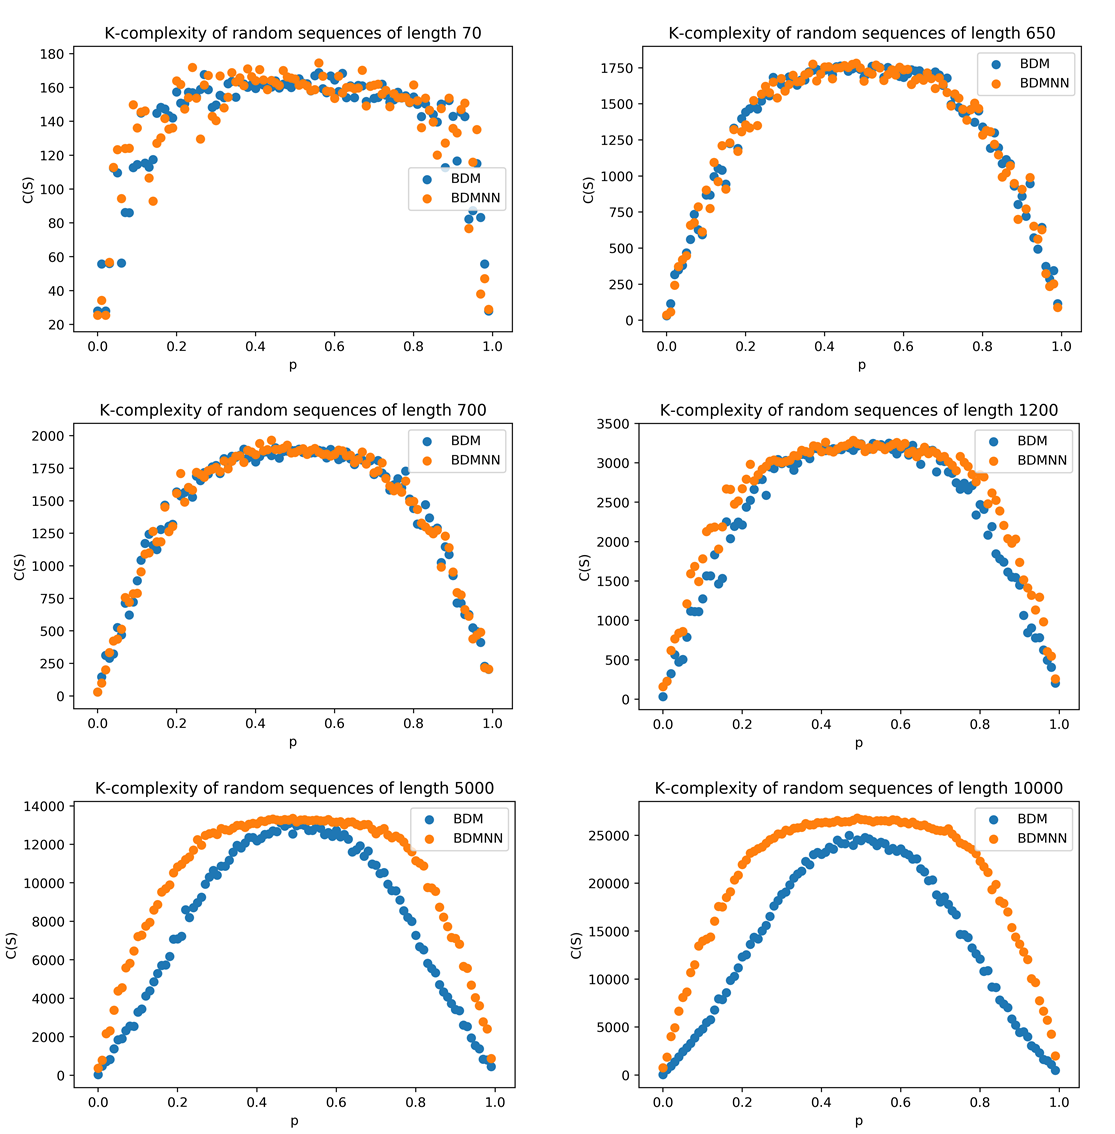
\includegraphics[width=\linewidth, height=\textheight,keepaspectratio]{seqs_BDMNN_result}
	\caption[The complexities of random sequences of bits, BDM versus BDMNN.]{The complexities of random sequences of bits of different lengths versus the probability parameter. The complexities were measured with the original Block Decomposition Method and with our proposal, the Block Decomposition Method with Neural Networks. The number of random sequences generated in each experiment was $100$.}
	\label{fig:seqs_BDMNN_result}
\end{figure}

We corroborated the previous, by performing this experiment with sequences of different lengths. The results are shown in Fig. \ref{fig:seqs_BDMNN_result}. As can be seen, the results obtained with our implementation, the BDMNN, showed a behavior which is pretty similar to the behavior and the results obtained with the BDM for sequences of length less than $1000$. This means that the regression performed by the Neural Networks was able to imitate the approximation to Kolmogorov complexity given by the original Block Decomposition Method. Nevertheless, for sequences whose size was greater than $1000$ bits, the results delivered by the BDMNN began to differ from the results of the BDM. We can see from the experiments with sequences of lengths $1200$, $5000$ and $10,000$ that the curve obtained with the BDMNN gets wider with the increase in the length of the sequences considered in the experiment.\\

The previous means that the error of the BDMNN increased with the size of the sequence considered, but moreover, we can see from the experiment shown in Fig. \ref{fig:10000_size_random_seqs} that the behavior of the BDMNN started to seem more like the behavior given by the techniques based on entropy or compression to measure complexity. Thereby, our method seemed to be capable of approximate the K-complexity with comparable results to the ones delivered by the BDM, moreover, it performed like the Shannon entropy for long sequences, for which it lost accuracy. This convergence to an entropic behavior also is present in the original implementation of the Block Decomposition Method (see \cite{decomposition}). Thus, it is natural that our implementation which is an imitation of the original BDM also should show this behavior. However, in the case of the BDMNN, it was amplified by the accumulation of error when predicting the complexity of the decomposed block sequences. This caused the entropic behavior to be manifested faster than it did with the BDM.\\

This does not mean that our proposal, the Block Decomposition Method with Neural Networks was inferior. It must be remembered that its initial purpose was to be a faster implementation to approximate the K-complexity. Therefore, if it proves to be faster than the BDM, it could become into a powerful alternative tool, especially because it could be used when it is possible and needed to sacrifice some accuracy of the approximation in exchange of speed in the computation.

\subsection{The Error and Computational Time of the BDMNN}
Now, we will try to show that our implementation works faster than the original Block Decomposition Method. To do so, we will perform an experiment to measure the computational time needed by both methods, the BDM, and the BDMNN, to measure the K-complexity of sequences of bits.\\

We will start by generating a random sequence of bits with a given length. This time it is not necessary to control its complexity, so the sequence will be randomly chosen among all the possible sequences of the given length with a uniform probability distribution. Then, we will measure its complexity with the BDM and the BDMNN. For both methods, we will perform a timing to determine the computational time needed to execute the function which computes the complexity with each method. The timing will be performed with the aid of the function $process \_ time$ which belongs to the library \textit{time} of Python. The resolution of this function, when implemented in Colab, was $1$ ns. Besides the timing process, we will compare the complexity computed by the BDMNN with the complexity computed by the BDM to determine the absolute error obtained with our method. We will perform this procedure starting with a sequence of length $12$, then we will perform it with a sequence of length $13$ and so on.\\

\begin{figure}
	\centering
	\begin{subfigure}[b]{0.8\textwidth}
		\centering
		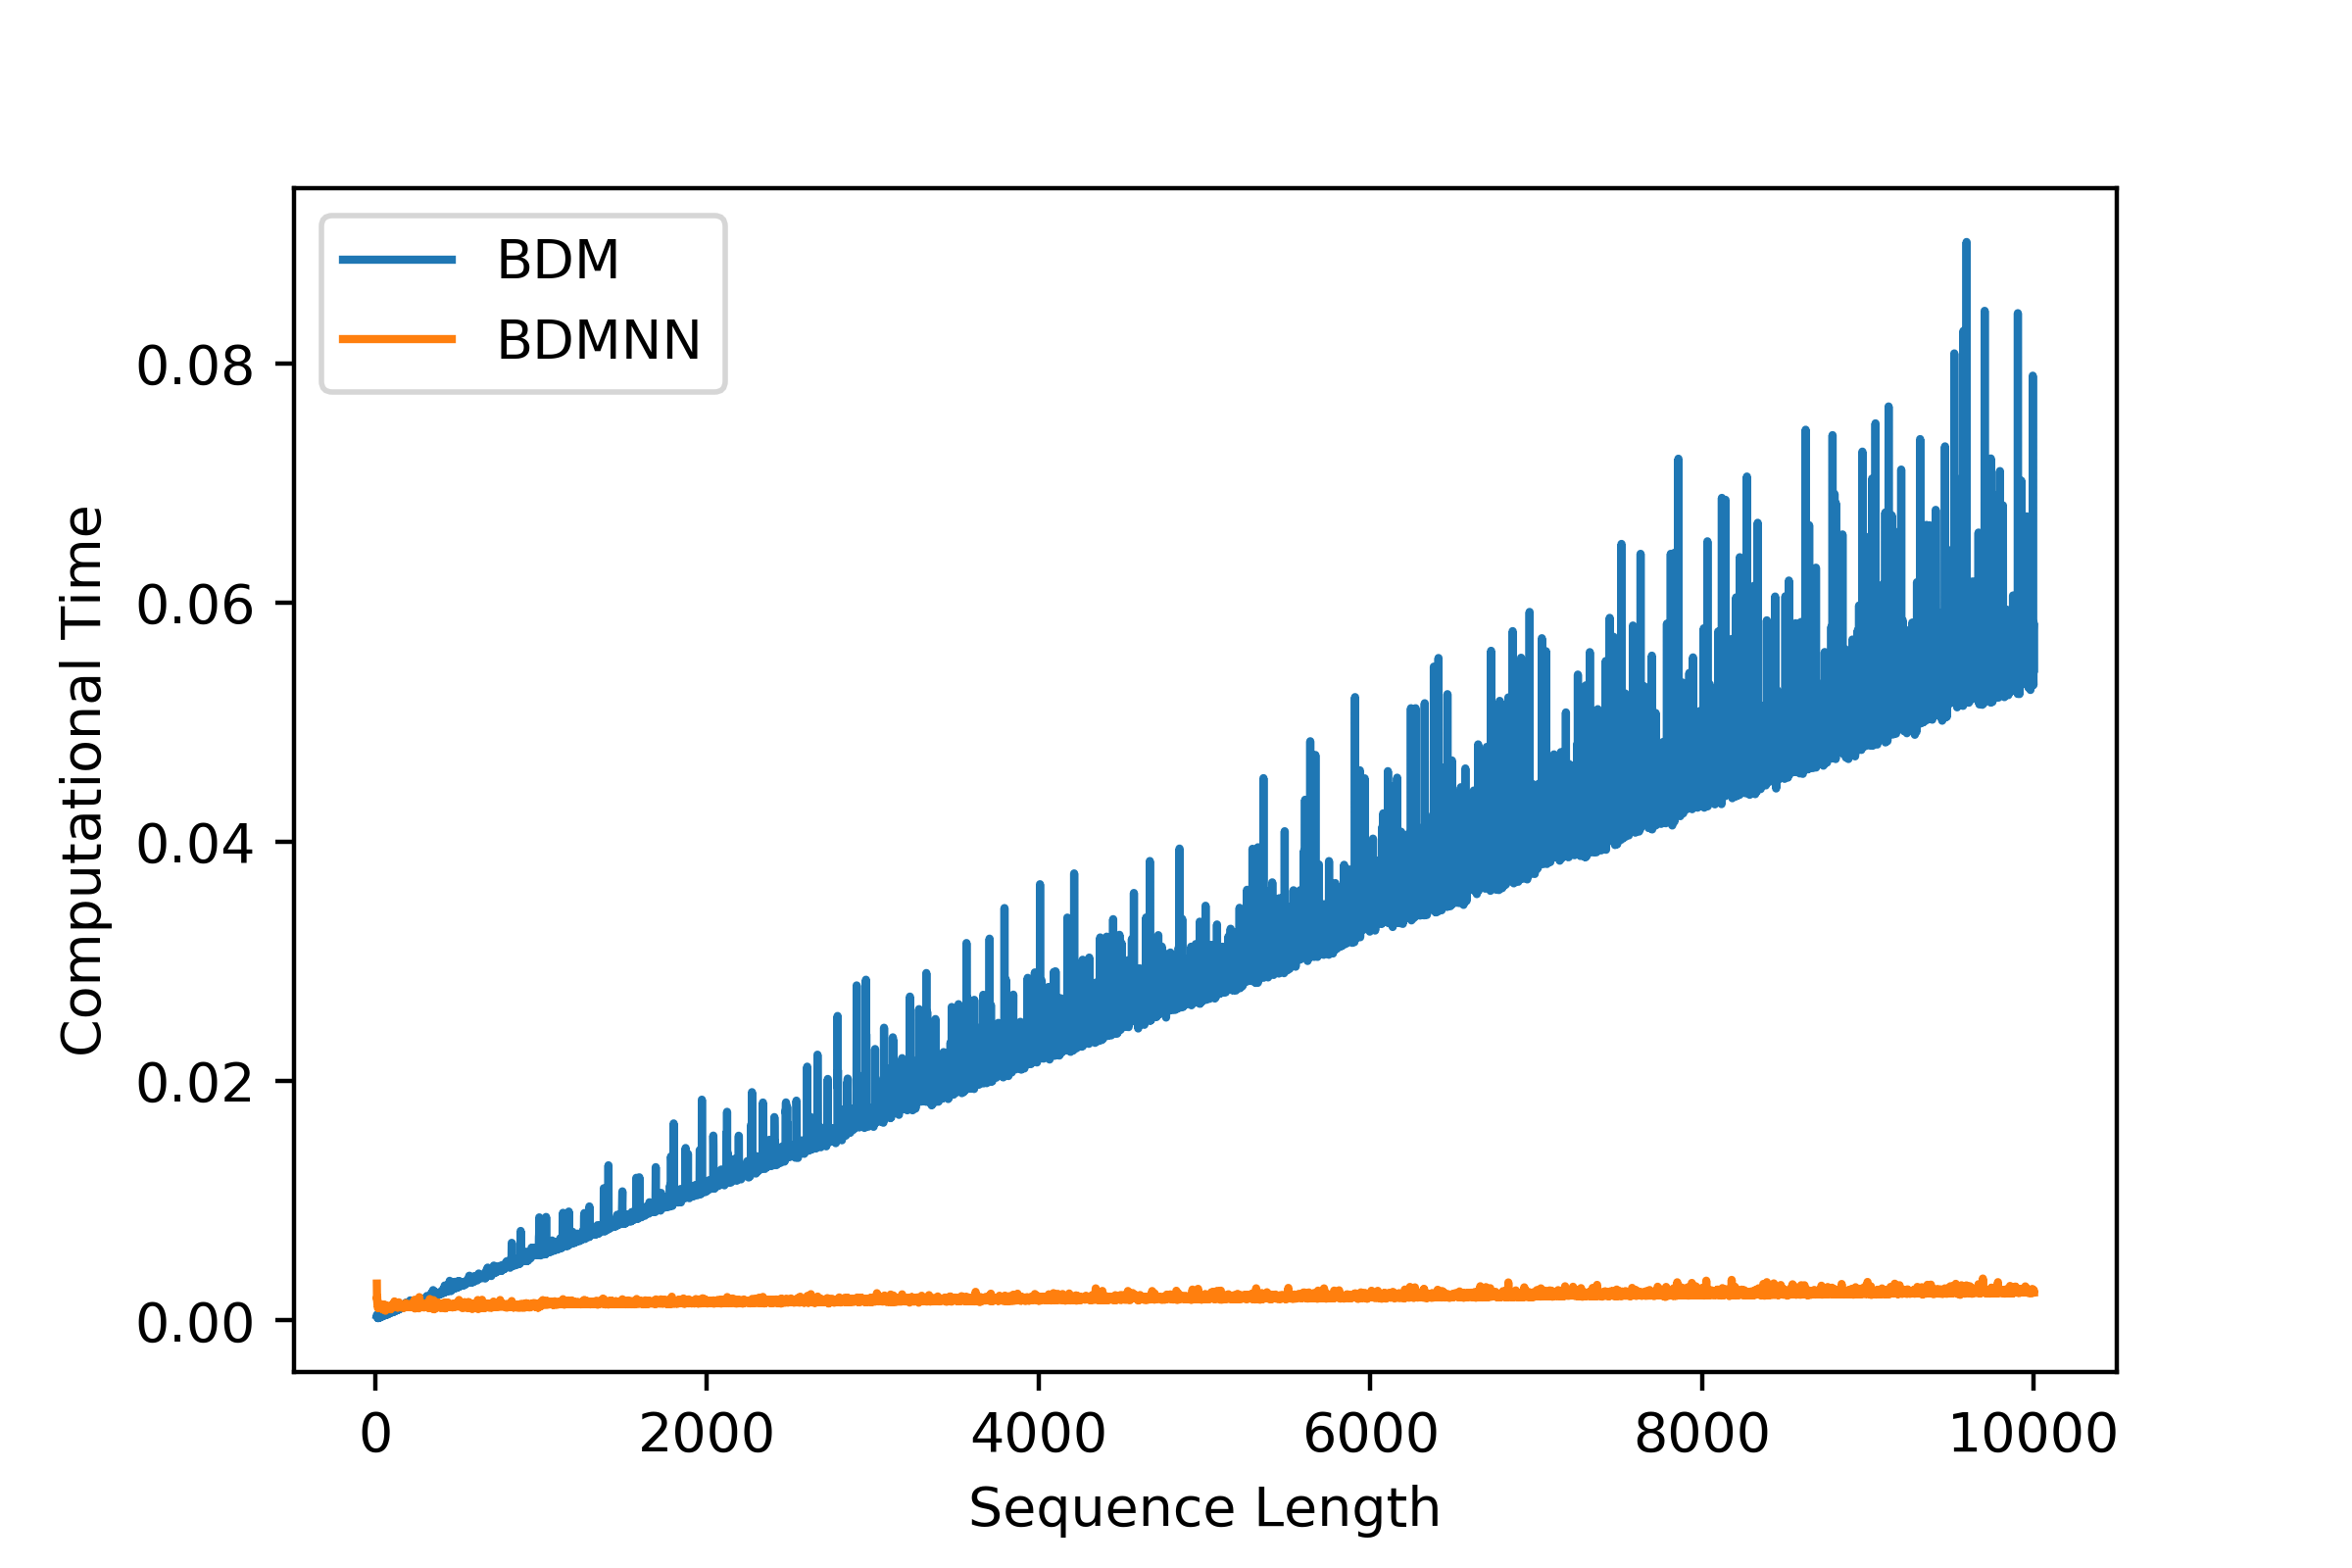
\includegraphics[width=\textwidth]{timing_results}
		\caption{}
		\label{fig:timing_results}
	\end{subfigure}
	%\hfill
	\hspace{0.001mm}
	\begin{subfigure}[b]{0.8\textwidth}
		\centering
		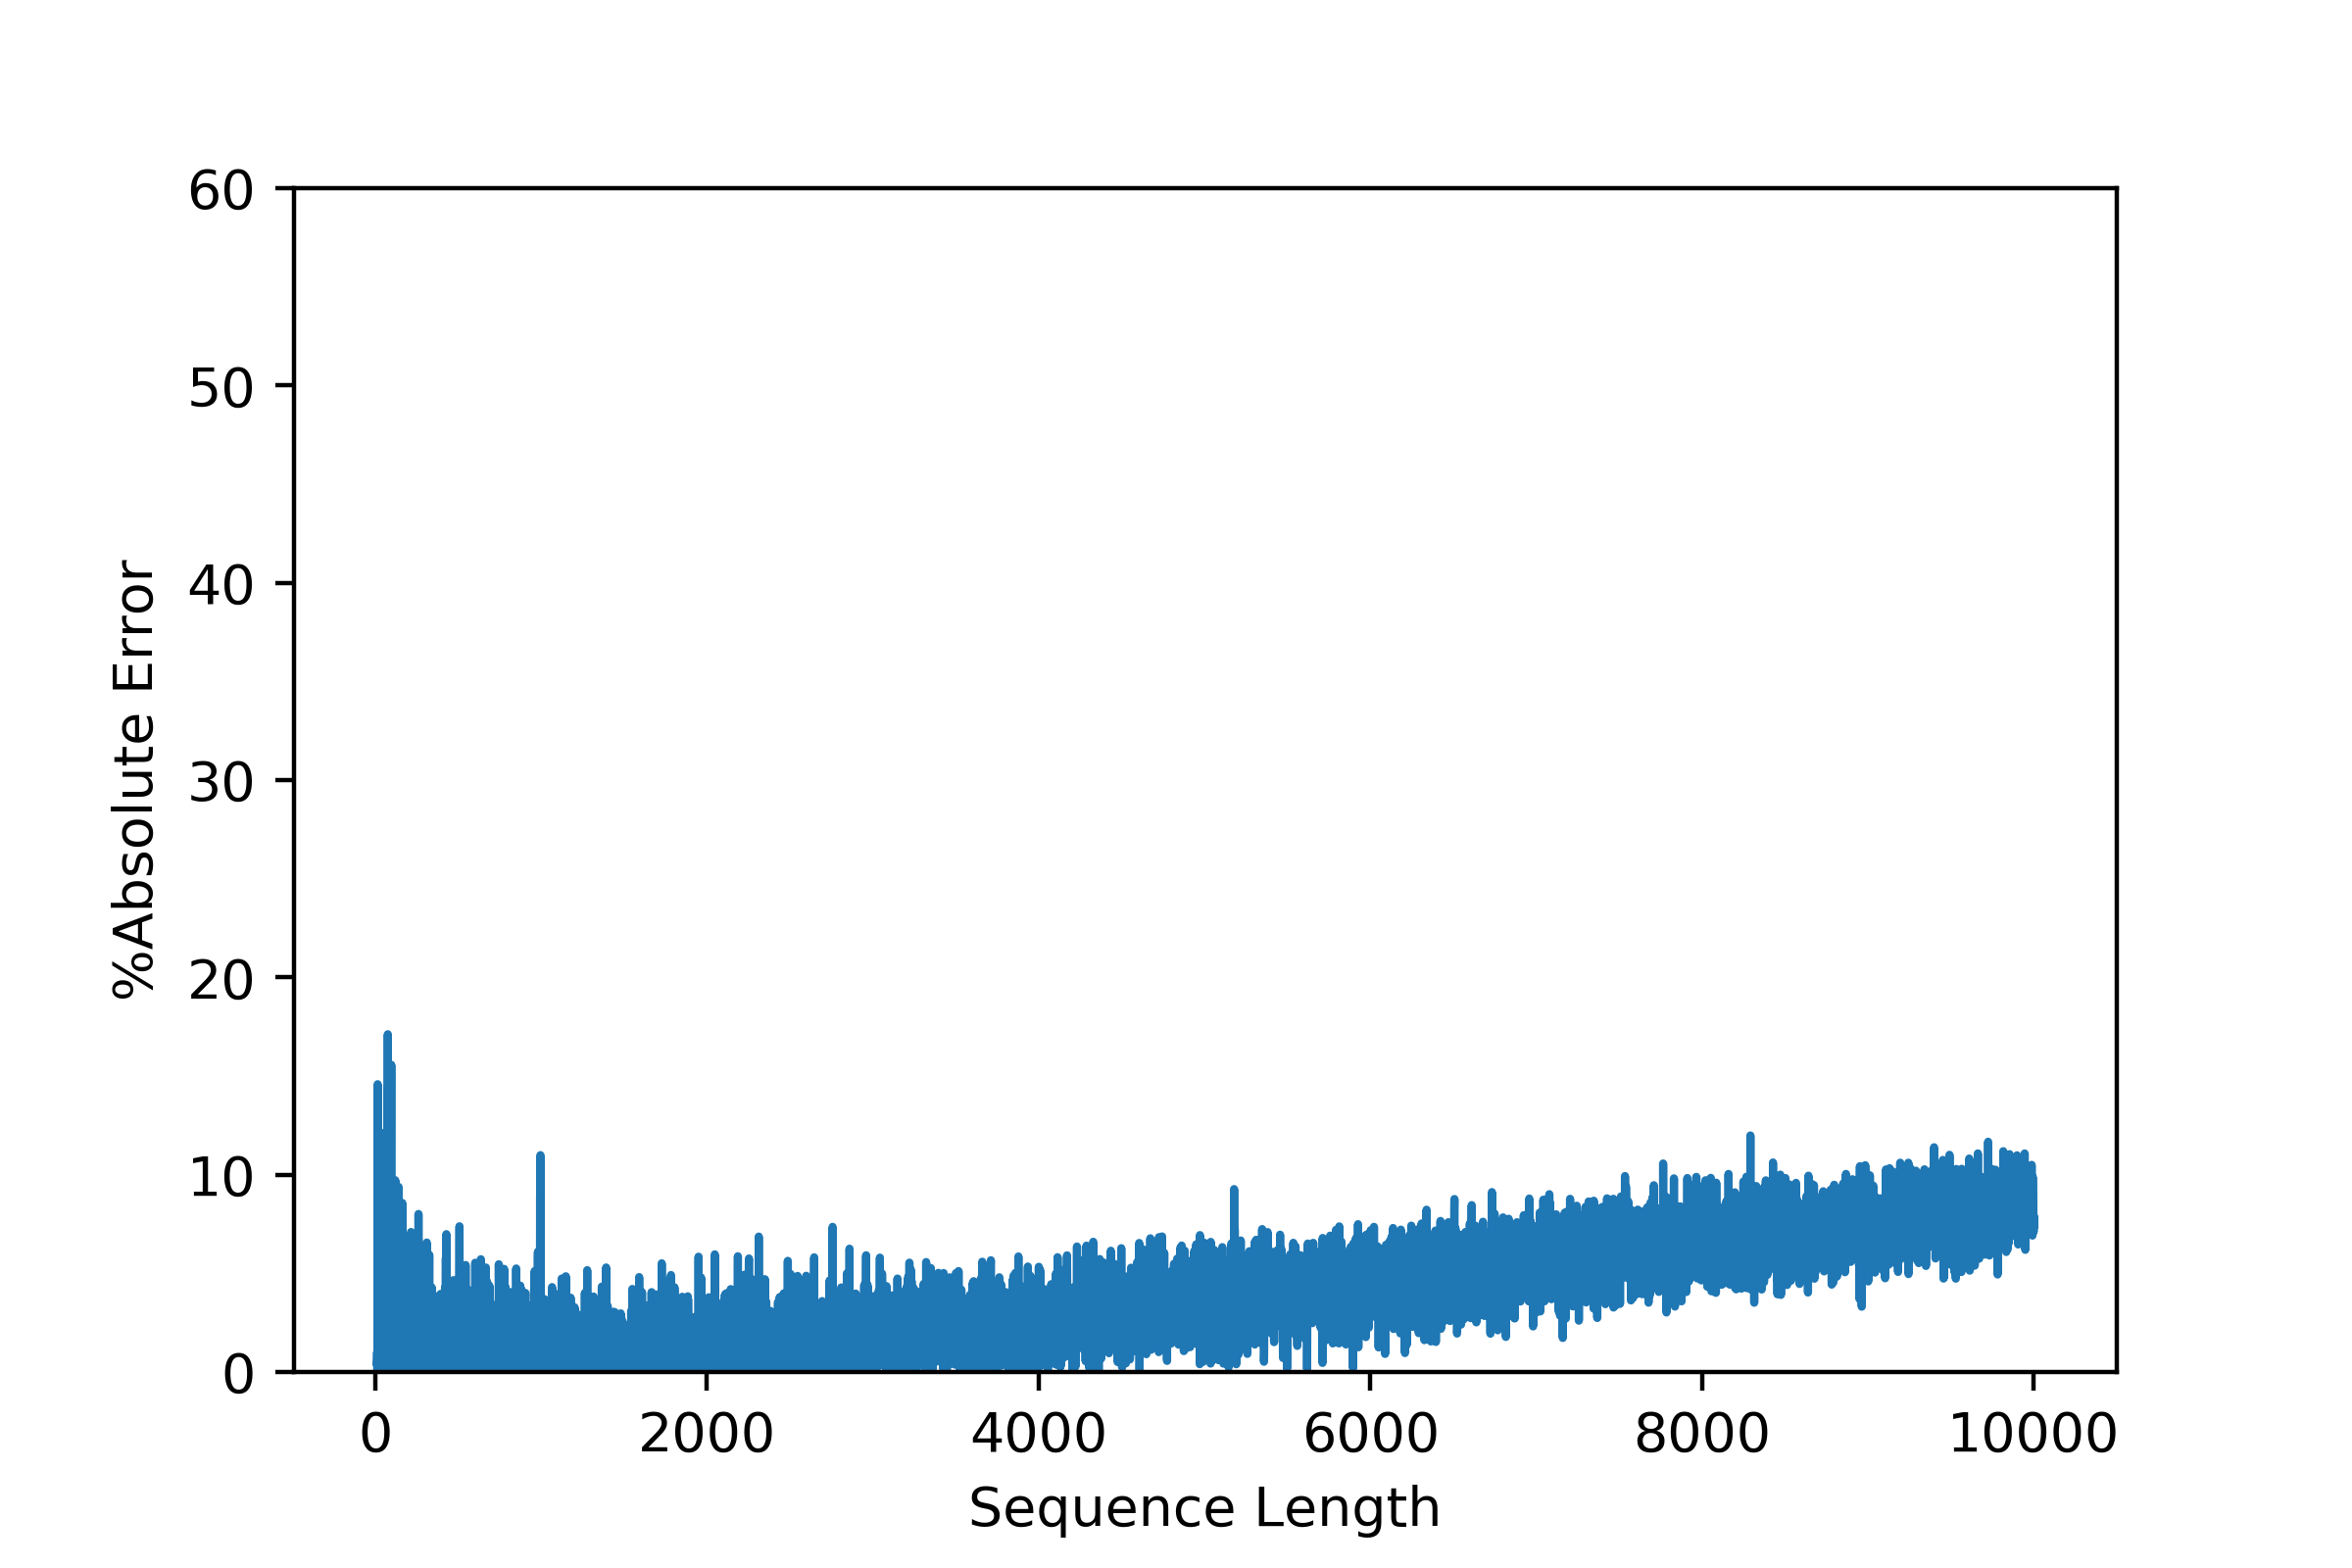
\includegraphics[width=\textwidth]{error_results}
		\caption{}
		\label{fig:error_results}
	\end{subfigure}
	\caption[Computational time and absolute error obtained with the BDMNN.]{(a) The computational time needed to implement the Block Decomposition Method (BDM) and the Block Decomposition Method with Neural Networks (BDMNN) to measure the K-complexity, versus the sequence length. The computational time is measured in seconds. (b) The percentage of absolute error of the complexity computed with the BDMNN compared with the complexity computed with the BDM, versus the sequence length.}
	\label{fig:tim_error_results}
\end{figure}

The results of this experiment are shown in Fig. \ref{fig:tim_error_results}. As can be seen in Fig. \ref{fig:timing_results}, this experiment showed as expected, that our implementation is faster than the BDM, moreover, the computational time of the BDMNN stayed constant with the sequence length, while it increased linearly for the BDM. Furthermore, the absolute error stayed bounded below $10 \%$ for sequences whose size was less than $4000$ with the only exception of the initial sequences for which the absolute error was around $17 \%$. For sequences with sizes larger than $4000$, the absolute error increased linearly. However, it increased slowly since for sequences of length $10,000$ its value was barely around $10 \%$.\\

These results have shown that our initial hypothesis was correct and the BDMNN computes faster the K-complexity. Moreover, the loss of accuracy occurs slowly with the length of the sequence and only is significant for very long sequences. This justifies its use for calculations were the computational time is important and the BDM takes so so long to be implemented that it becomes a restriction for the experiment.\\

The code to execute the experiment of this section can be found in the Appendix Section \ref{codes_python} (Fig. \ref{fig:timing_error_code}).

\subsection{The BDMNN Versus a Parallel Implementation of the BDM}
Now, we want to go further and evaluate the speed of our implementation versus a parallel implementation of the BDM. This parallel implementation is included in the library of the Block Decomposition Method for Python. This function splits the sequence and distributes the pieces into the available kernels. In this way, every kernel computes a piece of the process to accelerate the BDM.\\

This parallel implementation to compute the BDM was created with the objective of decrease the computational time needed approximate the K-complexity. In fact, this implementation was not available in the Wolfram Language implementation, so it is expected to be possibly one of the fastest possible implementations since Python by itself is a fast language. Hence, if we can beat this implementation, our implementation automatically could be considered the fastest implementation to compute the Kolmogorov complexity. Moreover, even if our implementation cannot beat the parallel implementation of the BDM, it still is possible to consider also a possible parallel implementation for the BDMNN.\\ 

We will repeat the same experiment of the last section, but this time instead of the classic BDM we will use this parallel implementation. The timing performed in the following experiment does not consider the time needed to divide the sequence into smaller sequences nor the distribution of them to the available kernels. The number of parallel kernels used was $4$.\\

\begin{figure}
	\centering
	\begin{subfigure}[b]{0.8\textwidth}
		\centering
		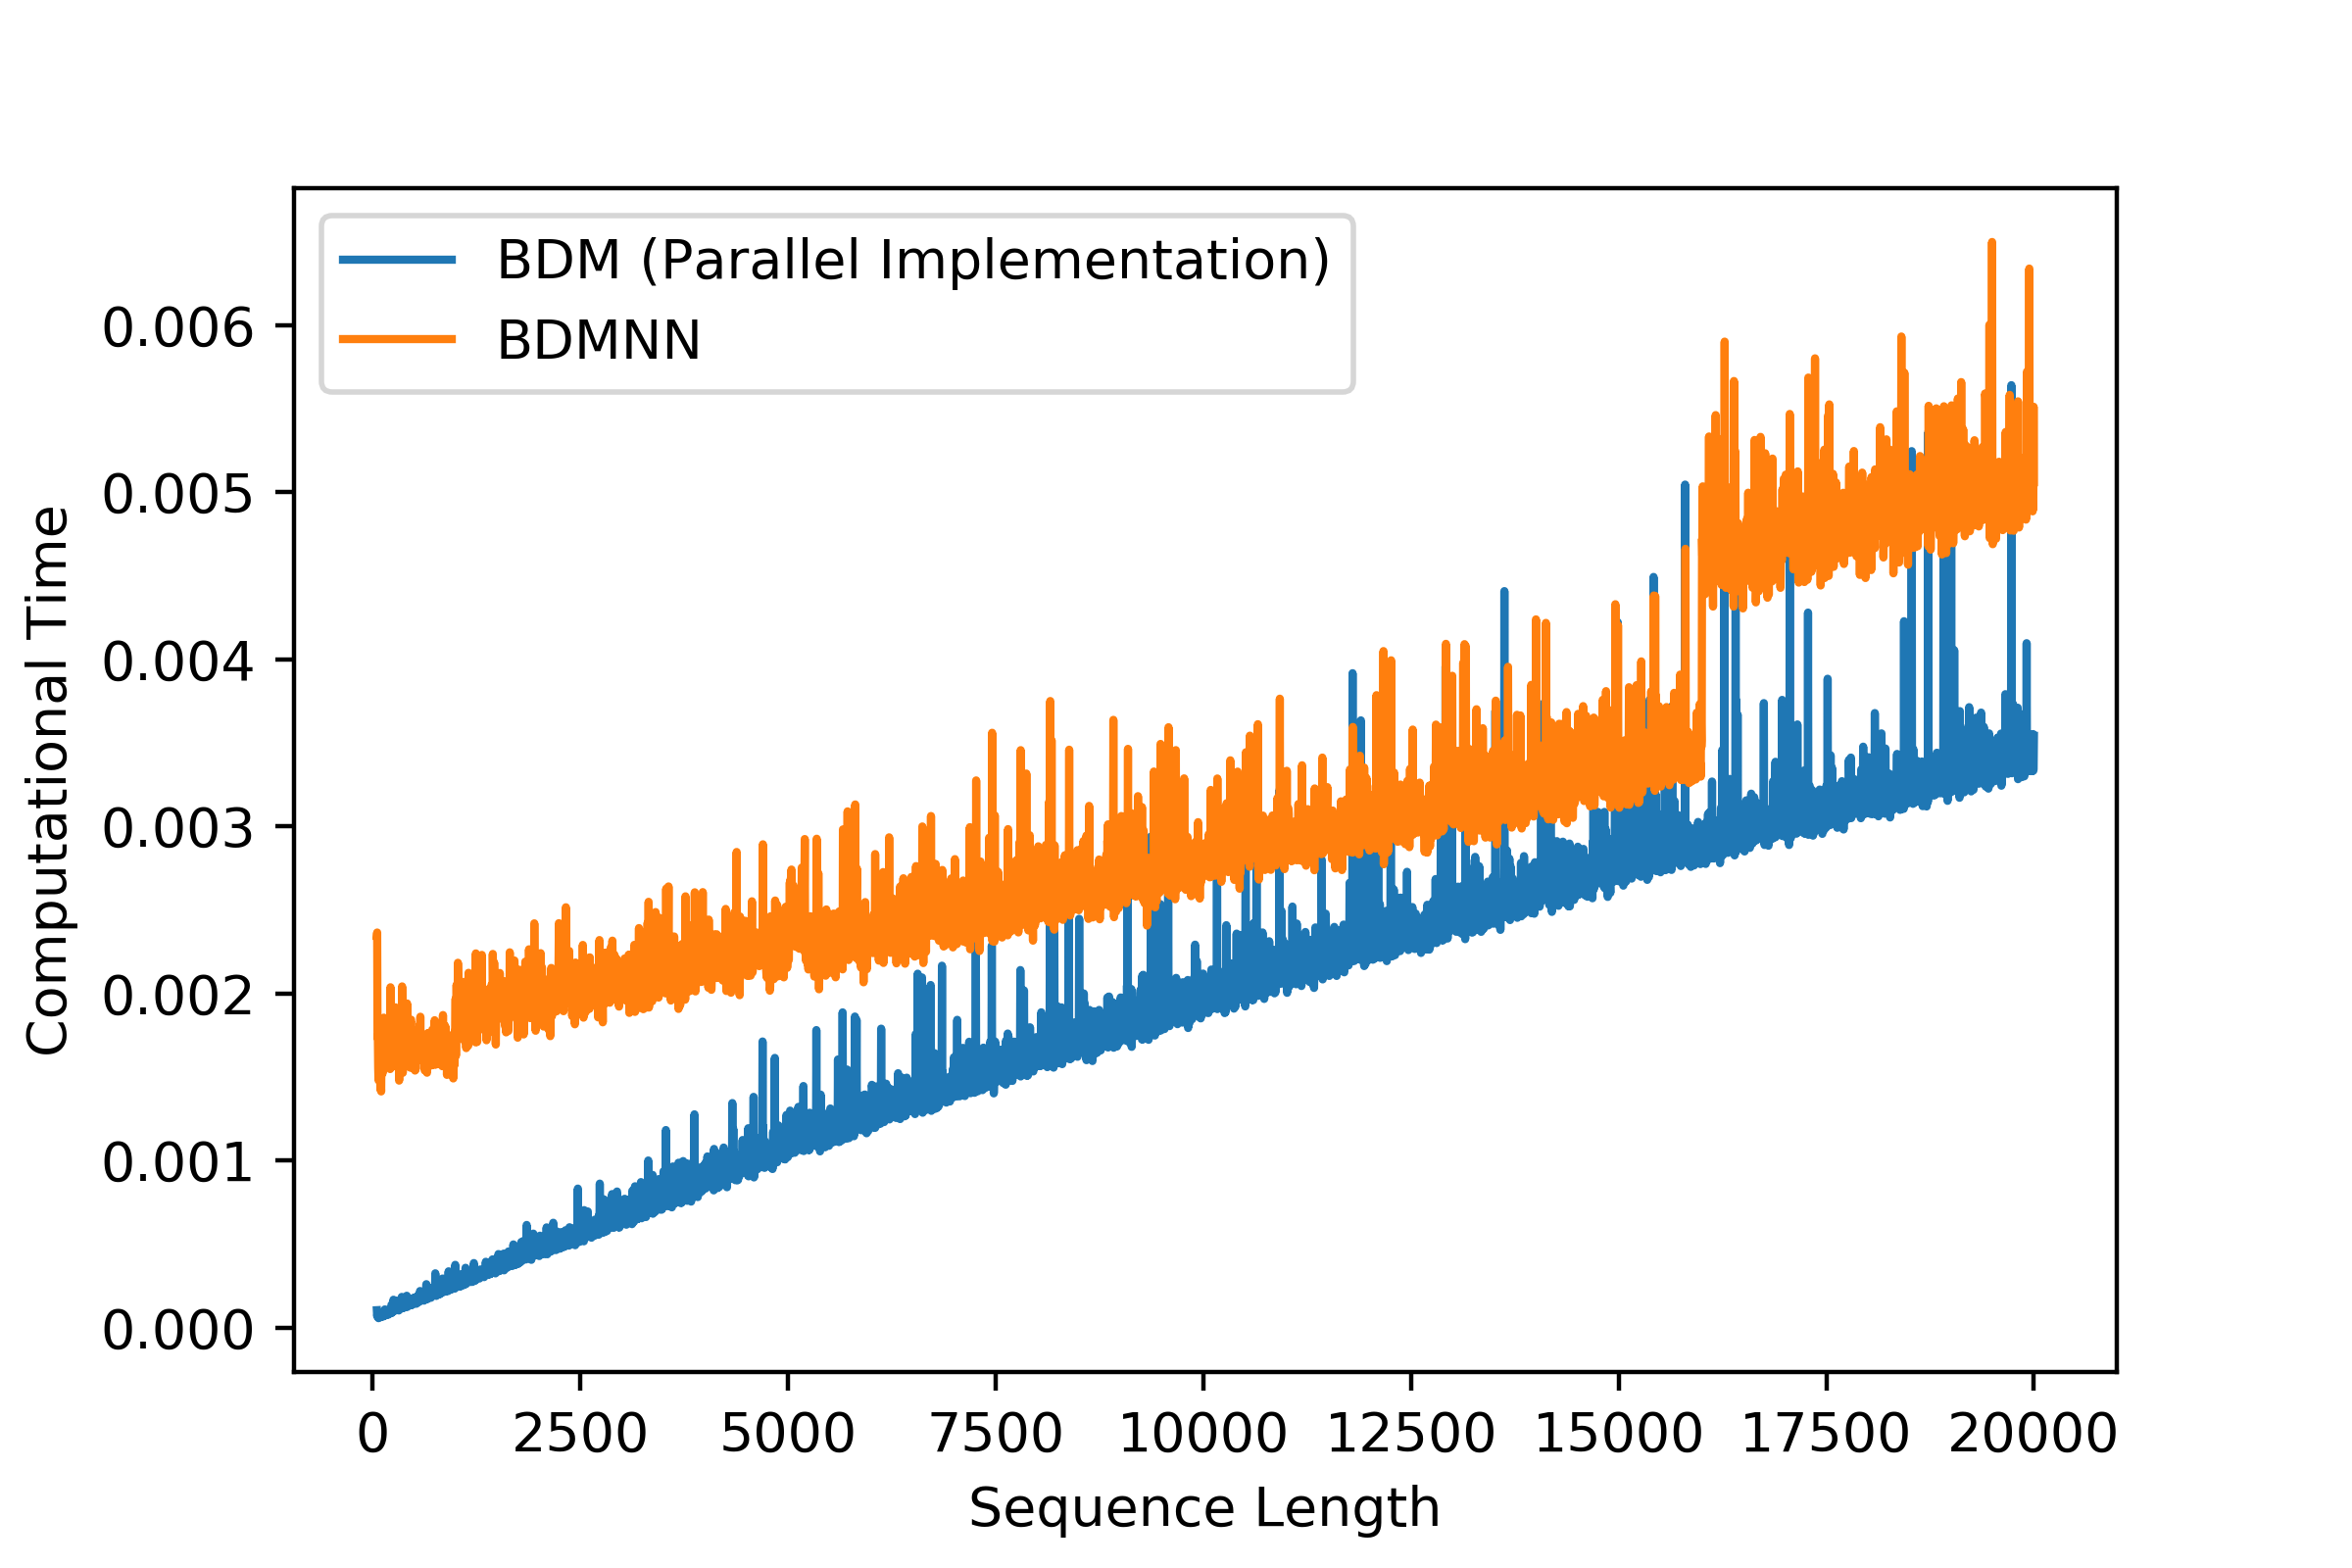
\includegraphics[width=\textwidth]{timing_results_parallel}
		\caption{}
		\label{fig:timing_results_parallel}
	\end{subfigure}
	%\hfill
	\hspace{0.001mm}
	\begin{subfigure}[b]{0.8\textwidth}
		\centering
		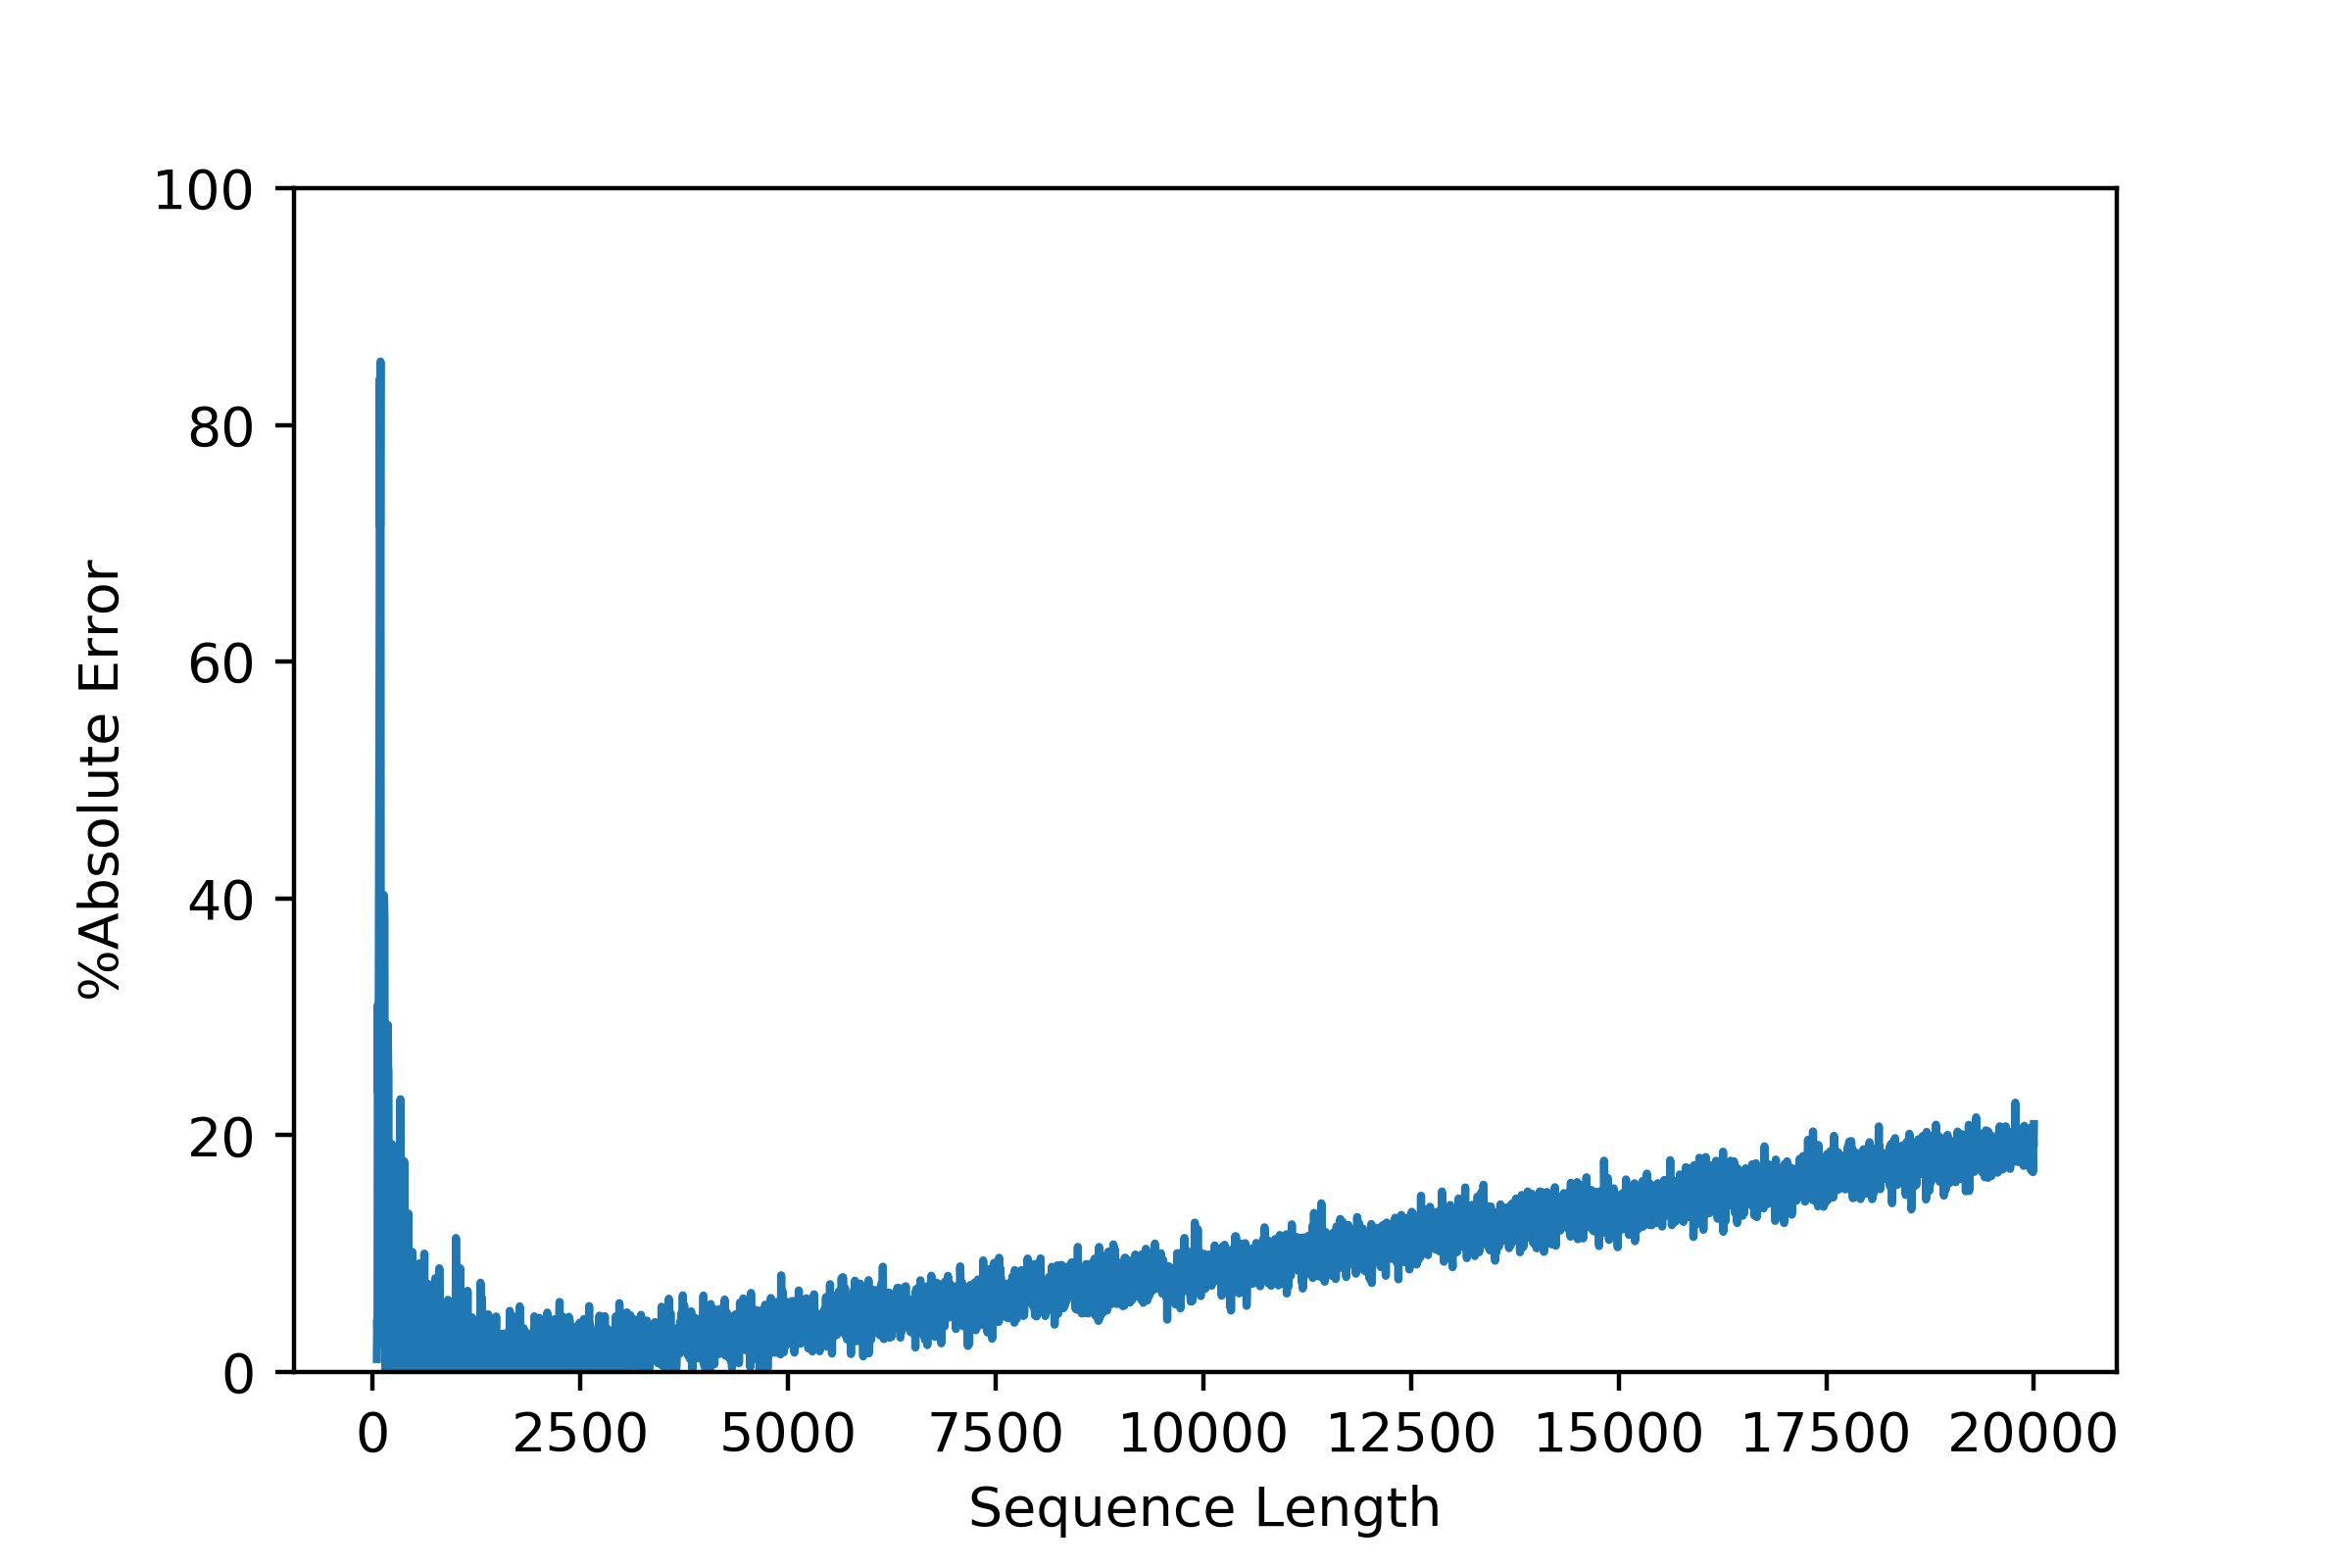
\includegraphics[width=\textwidth]{error_results_parallel}
		\caption{}
		\label{fig:error_results_parallel}
	\end{subfigure}
	\caption[Computational time and absolute error obtained with the BDMNN versus a parallel implementation of the BDM.]{(a) The computational time needed to compute a parallel implementation for the Block Decomposition Method (BDM) and the Block Decomposition Method with Neural Networks (BDMNN) to measure the K-complexity, versus the sequence length. The computational time is measured in seconds and for the parallel implementation, it does not consider the time needed to split and distribute among the available kernels the given sequence. (b) The percentage of absolute error of the complexity computed with the BDMNN compared with the complexity computed with the parallel implementation of the BDM, versus the sequence length.}
	\label{fig:tim_error_results_parallel}
\end{figure}

The results of this experiment are shown in Fig. \ref{fig:tim_error_results_parallel}. It can be seen in Fig. \ref{fig:error_results_parallel} that the absolute error obtained with the BDMNN showed a similar behavior that the absolute error shown in Fig. \ref{fig:error_results}. Nevertheless, the absolute error obtained with the initial sequences (short sequences with sizes of around $12$) was greater. This discrepancy not necessarily means that our implementation gave a big error for these short sequences. This result can be explained because the parallel implementation of the BDM has a different behavior for short sequences and since the Neural Networks of our implementation were trained with examples obtained from the original BDM, it was not expected the BDMNN to agree with the parallel implementation of the BDM. The parallel implementation of the BDM seems to have boundary problems for short sequences unlike the original BDM, so the result shown in Fig. \ref{fig:error_results} for short sequences was not alarming.\\

On the other hand, the result in Fig. \ref{fig:timing_results_parallel} showed that the computational time increased linearly for both methods. Nonetheless, the slope of this increase was very low for both methods. In fact, the BDMNN started with computational times larger than the computational times for short sequences with the parallel implementation of the BDM, however, the slope of the BDMNN was smaller than the slope of the parallel implementation for the BDM, thus, this would mean that for long sequences the BDMNN should overcome the parallel implementation. Nevertheless, for sequences whose size was around $16,000$ existed a jump in the computational time which made the computational time obtained with the BMDNN to increase. Even so, the parallel implementation of the BDM was just around $2ms$ faster than the BDMNN in the worst case. Thereby, a refined implementation for the BDMNN should easily overcome any implementation of the BDM.\\

Notwithstanding the previous results, we can argue that the former experiment was not fair since we did not take into consideration the time needed to divide the sequence into smaller sequences and to distribute them to the available kernels in the parallel implementation. For this reason, we repeated the experiment, but this time the timing for the parallel method included the time needed to split and distribute among the kernels the given sequence.\\

The result of this experiment is shown in Fig. \ref{fig:tim_error_results_parallel_2}. The results for the absolute error shown in Fig. \ref{fig:error_results_parallel_2} were the same as before. Nevertheless, the results in computational time were quite different. The results which are shown in Fig. \ref{fig:timing_results_parallel_2} showed that when we took into account the time needed to split and distribute the sequence among the available kernels, the parallel implementation was easily surpassed by our method, the BDMNN.

\begin{figure}
	\centering
	\begin{subfigure}[b]{0.8\textwidth}
		\centering
		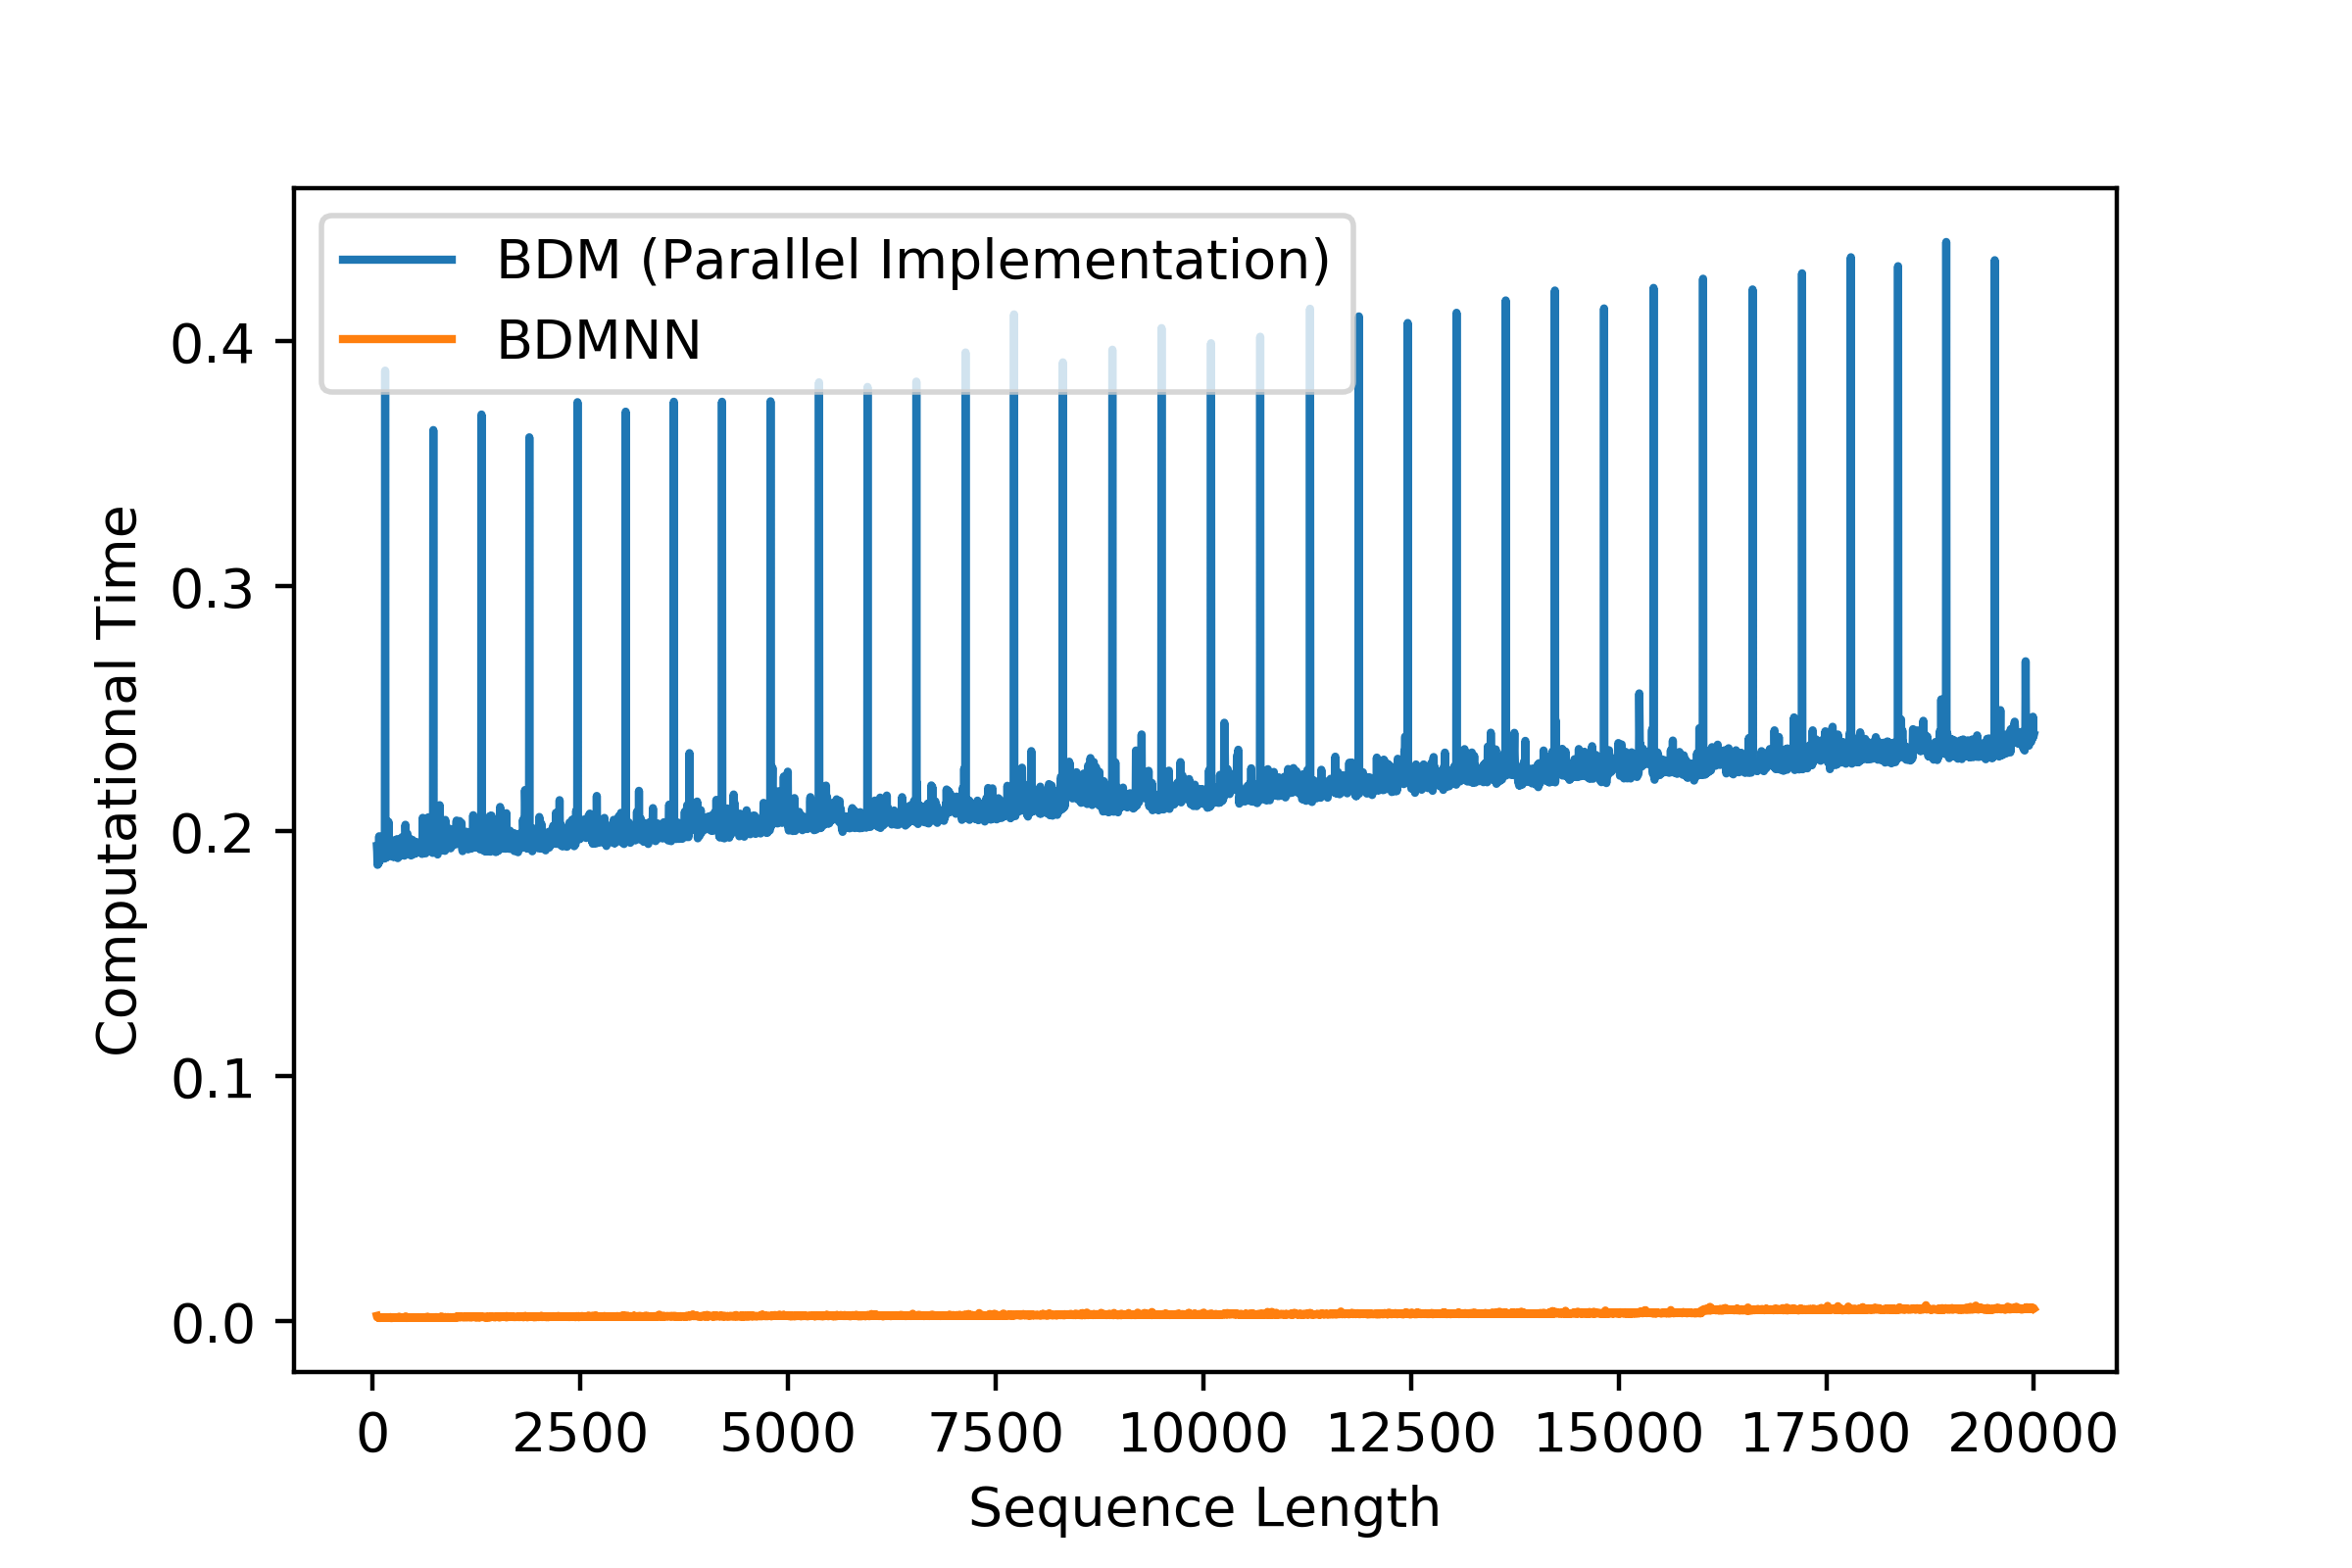
\includegraphics[width=\textwidth]{timing_results_parallel_2}
		\caption{}
		\label{fig:timing_results_parallel_2}
	\end{subfigure}
	%\hfill
	\hspace{0.001mm}
	\begin{subfigure}[b]{0.8\textwidth}
		\centering
		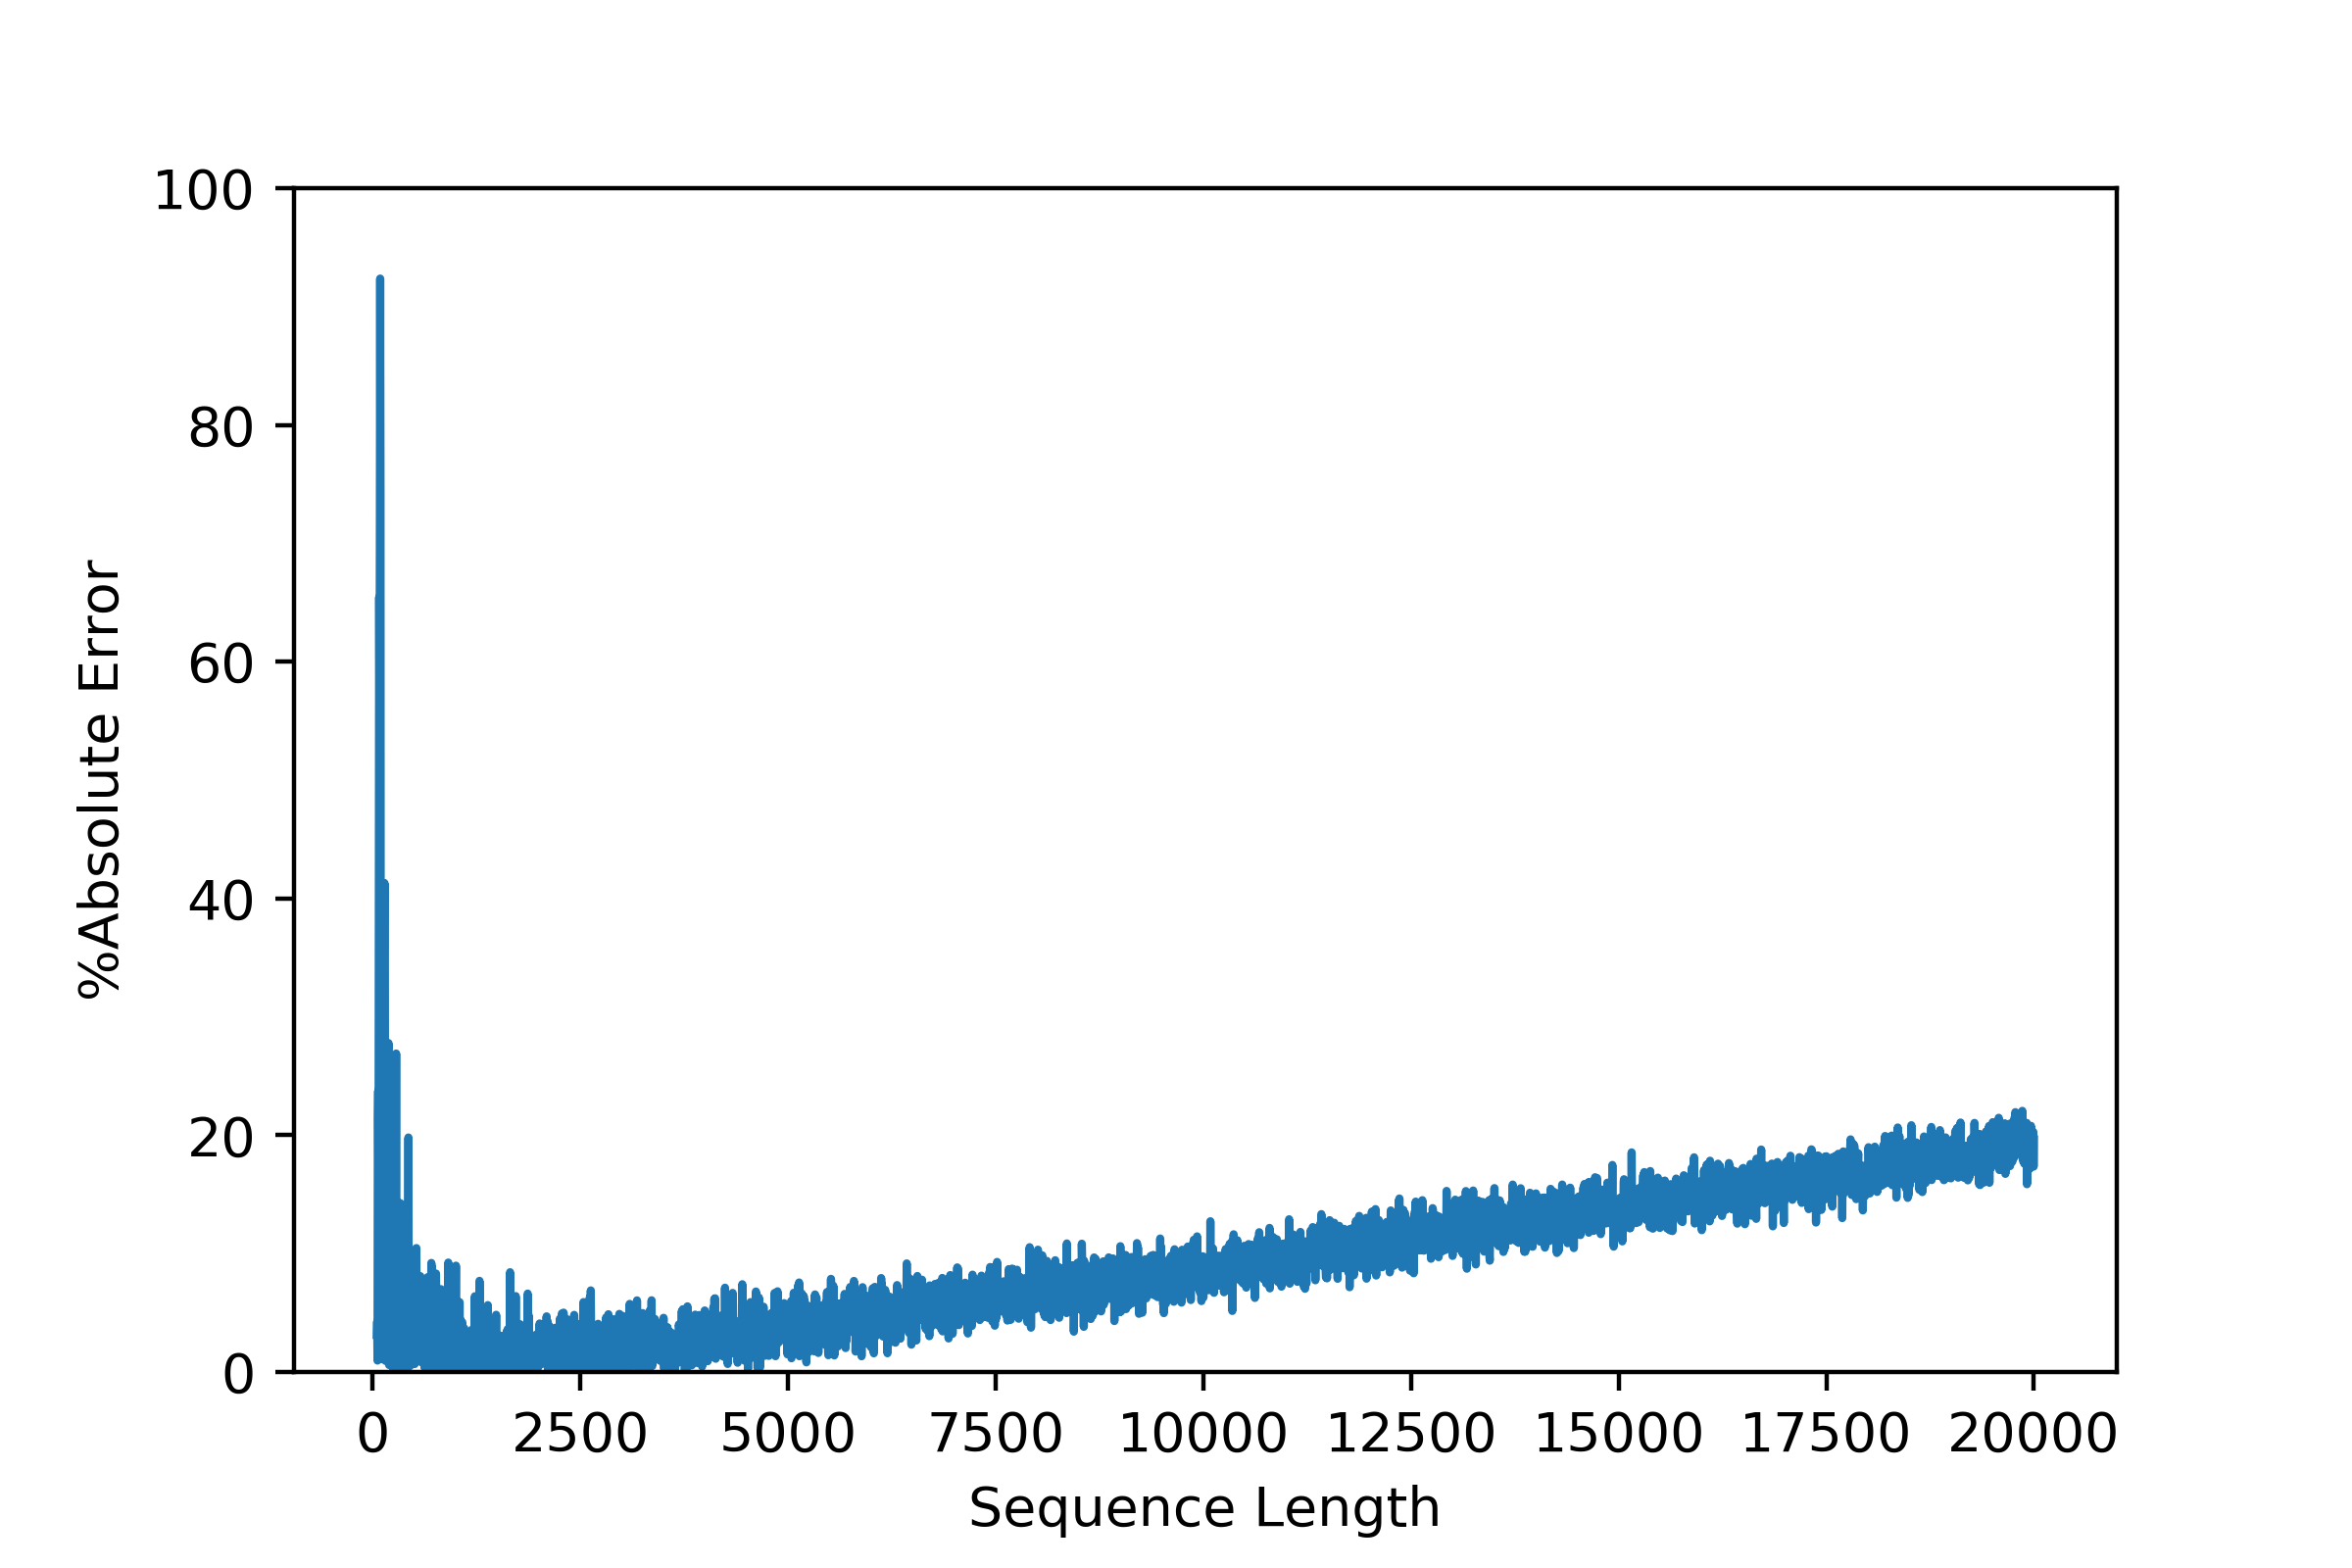
\includegraphics[width=\textwidth]{error_results_parallel_2}
		\caption{}
		\label{fig:error_results_parallel_2}
	\end{subfigure}
	\caption[Computational time and absolute error obtained with the BDMNN versus a parallel implementation of the BDM.]{(a) The computational time needed to compute a parallel implementation for the Block Decomposition Method (BDM) and the Block Decomposition Method with Neural Networks (BDMNN) to measure the K-complexity, versus the sequence length. The computational time is measured in seconds and for the parallel implementation, it does consider the time needed to split and distribute among the available kernels the given sequence. (b) The percentage of absolute error of the complexity computed with the BDMNN compared with the complexity computed with the parallel implementation of the BDM, versus the sequence length.}
	\label{fig:tim_error_results_parallel_2}
\end{figure}

The code to execute the two former experiments can be found in the Appendix Section \ref{codes_python} (Fig. \ref{fig:timing_error_code_2}).

\section{Conclusions}
The results obtained with our proposal, the Block Decomposition Method with Neural Networks (BDMNN), were outstanding, considering the simplicity of the idea behind it. It showed by far, to be faster than the original Block Decomposition Method. It even competes in speed with the parallel implementation of the BDM. The loss in the accuracy is not significant and remains below $20 \%$ of the absolute error for sequences with sizes below $20,000$ bits. In the worst cases, its behavior resembles an entropic like behavior.\\

We strongly believe that this method can be improved even further. We could reduce the error by enhancing the training of the Neural Network models by means of more data examples, more training time, a more sophisticated model, or even another regression technique could be considered. Also, better programming of the block decomposition algorithm could help. For example, by considering an overlapping parameter or the use of more neural networks to perform more refined predictions. Finally, a parallel implementation with Neural Network models should render spectacular timing results.\\

The original Block Decomposition Method uses the complexity results for sequences whose length is equal or less than $12$ to compute the complexity of larger sequences. Instead, our method uses the complexity results for sequences whose length is in between $12$ and $1000$, to extend them to larger sequences. Therefore, both methods are basically the same, the only difference is the size of the sequences whose complexity is known. In the case of the BDM, its complexity was computed from the Coding Theorem Method (CTM), and in the case of the BDMNN, its complexity is computed from the regression performed by Neural Networks.\\

In the end, our method can be used as a good approximation to Kolmogorov complexity, especially when the computational time is important, and we do not care to lose some accuracy in the results.

%basicamente lo que hago con la red neuronal, es aumentar %el tamaño minimo de secuencia en el método bdm, ya que %este metodo solo puede trabajar con secuencias de %longitud 12, entonces yo hago una regresion para poder %trabajar con long minima hasta 1000, lo que disminuye la %cantidad de tiempo al necesitar evaluar menos %subsecuencias obtenidas al cortar la secuencia


%ver y poner subrayado en azul en articulo le defi des %faibles complexites y en articulo a decomposition. este %problema justifica la busqueda de un metodo menos costoso %comptacionalmente para calcular la complejidad de kolmo
%también lo surayado en azul en art de los universos a la %mente
%tambien lo encerrado en rosa en art des faibles pag. 84
%poner lo subrayado y marcado con doble ** en pag 2 de art on measuring the complex of networks

%sin embargo ver subrayado en azul pag. 4 a decomposition %method